\chapter{\VBFHBB\, Analysis}\label{c:K}

	After comparing the base constituents of the \VBFHBB\, event between the offline and HLT level and finding them to be similar in behaviour, the specific objects that make up a \VBFHBB\, event can be studied and compared. In this section, the events were required to pass all cuts discussed in Section \ref{es:as} and the designation of the jets as $b_i$, $j_i$ is highlighted in that section.


\section{Cutflow}
\label{k:cutflow}

	Prior to investigating the core kinematic variables and the more complex kinematic variables used for the Boosted Decision Tree training (Appendix \ref{a:bdt}), the event cutflow for both the Monte-Carlo and real data should be studied to highlight any differences between the event counts. The event counts are given in Table \ref{t:cutflow}, and the ratio of the events is shown in Figures \ref{f:cutflowD} and \ref{f:cutflowMC}.

	\begin{table}[h]
		\caption{Cutflow for the \textit{two-central} \VBFHBB\, events as described in Section \ref{es:as}. The cutflows are given for the online and offline channels in both data and Monte-Carlo along with the percentage of original events.}
		\label{t:cutflow}
		\medskip
		\centering
		\begin{tabular}{c|c|c|c|c}\toprule
			Cut & MC Offline & MC Online & Data Offline & Data Online \\\midrule
			Clean Events & 6229.48 & 6229.48 & 150611000 & 150611000 \\
			Trigger & 6229.48 & 6229.48 & 6679390 &  6679390 \\
			$\geq2$ \textit{loose} \bjets & 503.552  & 467.146 & 2275760 &  2932620 \\
			$\geq2$ light-jets & 483.499  & 417.845 & 2189700 &  2671280 \\
			\textit{Tight} \bjet\, requirement & 330.962  & 288.806 & 1490320 &   1640290 \\
			Forward jet requirement & 51.843   & 40.8484 & 1186610 &  958414  \\
			\ptbb$>160$GeV & 32.7426  & 26.7038 & 309454  &  259411  \\
			\bottomrule
		\end{tabular}
	\end{table}

	\subsection{Monte-Carlo}
		\begin{figure}[h]
			\centering
			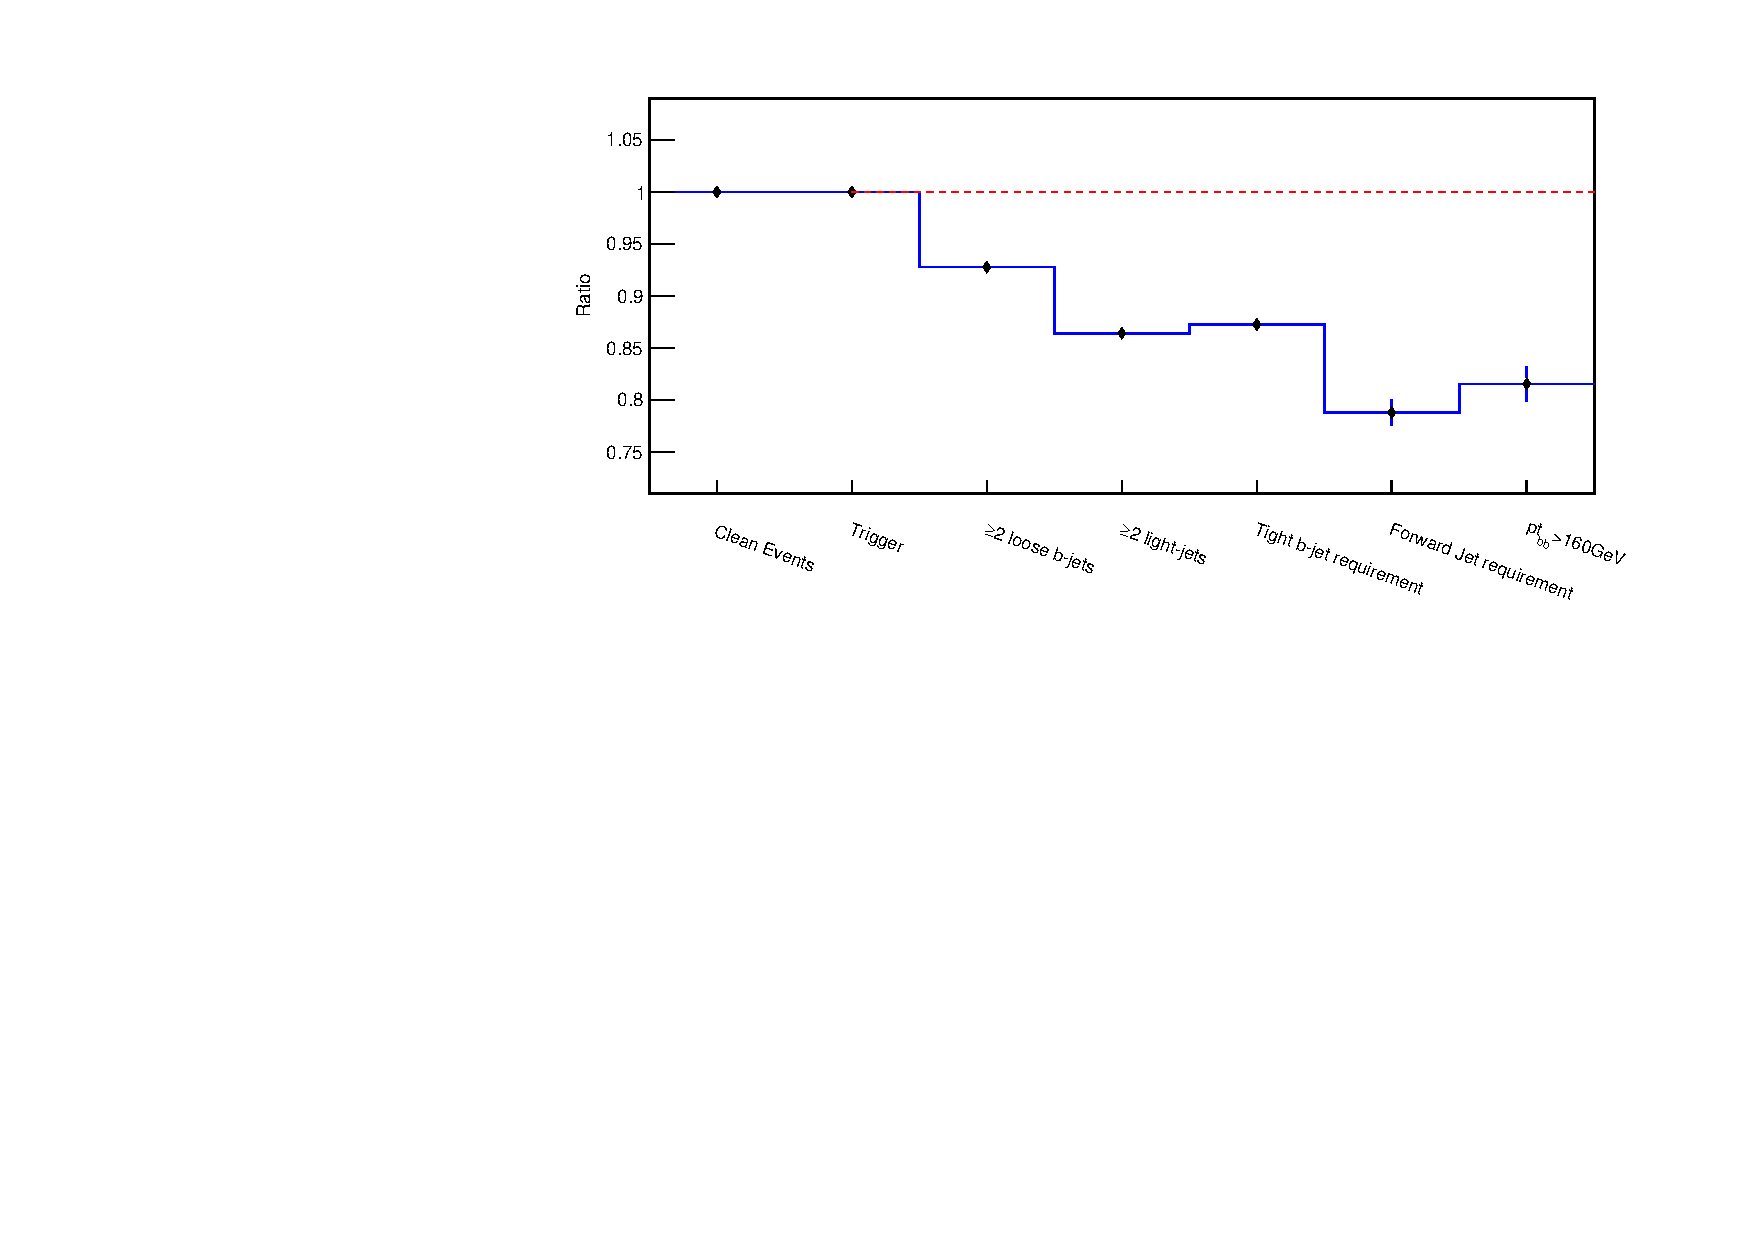
\includegraphics[width=0.75\linewidth]{MC_cutflow}
			\caption[\VBFHBB\ Cutflow ratio for Monte-Carlo simulation]{Ratio of the online event count over the offline event count for the Monte-Carlo}
			\label{f:cutflowMC}
		\end{figure}

	Overall, the online performance has fewer events than the offline for all points in the cutflow, and overall produces $\sim80\%$ of the total signal events. There are three distinct jumps in the cutflow ratio, at the cuts on the \textit{loose} \bjets\,, light-jets and the forward jet requirement, of $\sim7\%$ each. As shown in Figure \ref{fig:MC:bjetefficiency}, online \btag\, is $\sim93\%$ as efficient as the offline \btag. When considering tagging two distinct \bjets\,, any difference in efficiency is squared. Given the difference in tagging rates, this would result in $\sim86\%$ tagging efficiency for two \bjets\,, which is lower than shown in the cutflow. As shown for the leading \bjet in Section \ref{OP:leadingb}, the offline jet is typically higher in \pt than the online jets. However the difference is small , $\sim2\%$, so any effect on the cutflow should not be as pronounced.

	The $\sim7\%$ drop on the light jet requirement is unexpected, the requirement was solely for 2 jets with \pt$>20$GeV. Given the points above with respect to the \pt difference between online and offline, this drop should not be so sever. The fact the \pt cuts on the light jets were so low also suggests an anomalous result here as such a cut should not contribute a significant reduction in either online or offline.

	Following the drop for the light-jet cut, there is an unexpected increase in the online ratio following the \textit{tight} \btagging\, cut. As highlighted, the tagging efficiency was worse for online than offline, so any requirement for a tagged \bjet\, would be expected to produce a decrease in the online event count relative to the offline count. Perhaps spuriously, the cutflow at this point corresponds to the $86\%$ figure expected given the relative tagging efficiency for two \bjets.

	The final drop occurs following the requirement for a high \pt forward jet. Figure \ref{fig:O:leadingnonbptslice} shows that for non \bjets\, in the forward region of the detector, the \pt of the offline jet is consistently higher than the online \pt. This difference would result in a drop in the online events, with fewer jets passing the threshold \pt cut compared to the offline events.

	Overall for the Monte-Carlo events, there was a 20\% reduction in the number of events that passed the \VBFHBB\, cuts.










	\subsection{Data}
		\begin{figure}[h]
			\centering
			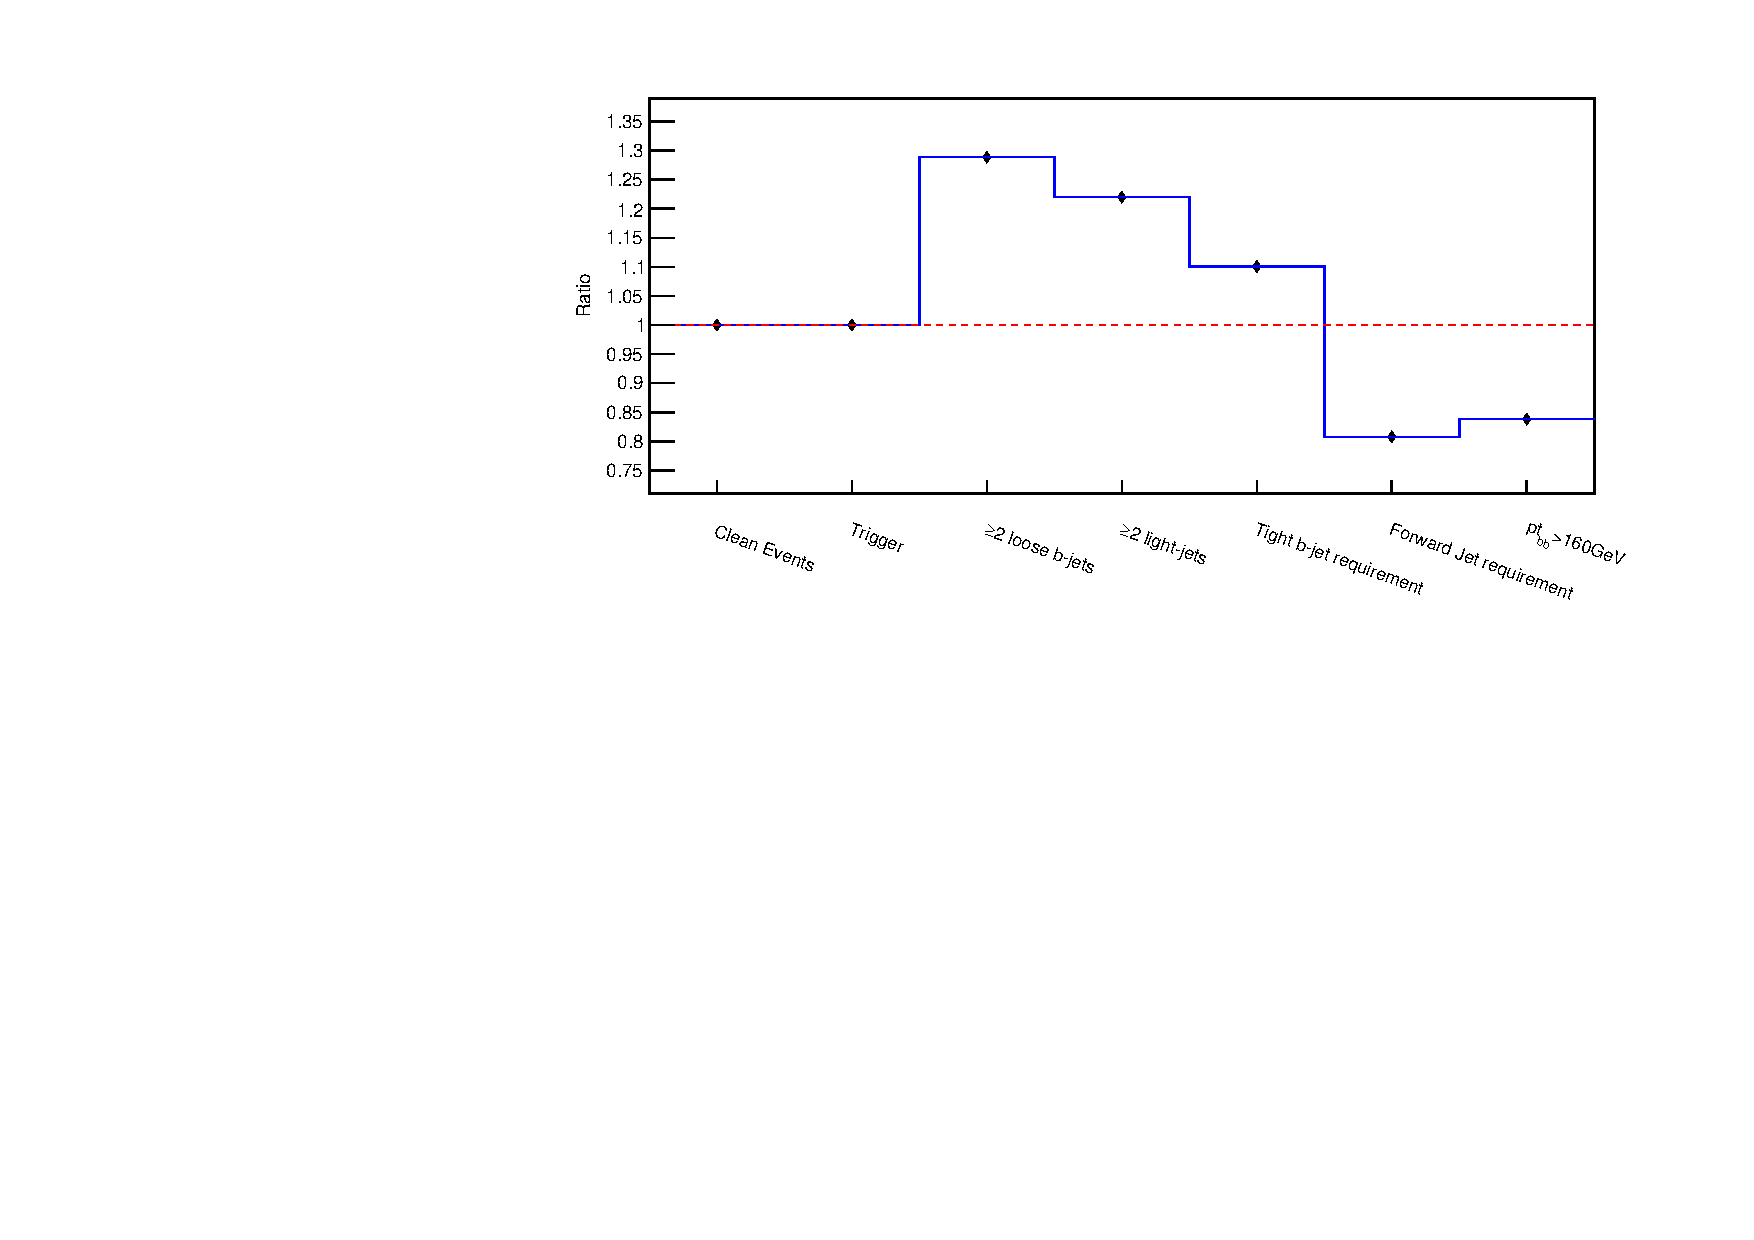
\includegraphics[width=0.75\linewidth]{D_cutflow}
			\caption[\VBFHBB\ Cutflow ratio for data]{Ratio of the online event count over the offline event count for the real data}
			\label{f:cutflowD}
		\end{figure}


	\subsection{Summary of Cutflow Comparison for the Online and Offline \VBFHBB\ events}

	While the granular details of the cutflow (LEAVE A LOT TO BE DESIRED), the overall effect on the reduction of events to the final \VBFHBB\ event state is consistent between both the Monte-Carlo simulations and data.

	The final relative reduction in online event count relative to the offline event count is shown for the Monte-Carlo simulations in Figure \ref{f:cutflowMC} to be to $\sim82\%$ of the offline event count. Similarly the ratio plot for the data events in Figure \ref{f:cutflowD} results in $\sim84\%$ final state events for the data events. The consistent values for the rate reduction of a trigger-object based analysis suggest that future analyses may be able to apply TLA to the \VBFHBB\ channel to increase the event yield in these analyses and improve the statistical significance of any results.

	With an average $\sim83\%$ reduction in event rate for the channel, usage of TLA at a rate of $2$kHz as described in Ref. \cite{TLA} and Section \ref{t:tla} would result in an increase in output events of $\sim66\%$ compared to a standard offline analysis.

	This statement is an estimate, there is additional computational cost involved with storing and computing the quantities required for the \VBFHBB\ analysis, such as the increased event size mentioned in Section \ref{obp:beff} as a result of storing the \btag\ training quantities to apply the updated algorithms. A rate analysis to ensure the TLA can be applied in the \VBFHBB\ channel without decreasing the rate increase down to the point the final TLA event count is no longer an improvement is a necessary step before approving TLA, but is beyond the scope of this dissertation.


\section{Specific Jet Feature Distributions}
\label{k:jets}

	While the previous chapter showed that the \bjets\ and non-\bjets\ had slight differences that could be rectified for future analyses, the behaviour is sufficiently similar that plots of the kinematic quantities of the \VBFHBB\ jets can be made to ensure behaviour is consistent for the specific jets that make up the final state from Table \ref{t:cutflow}.

	\begin{table}[h]
		\caption[Signal/Background definition \mbb values]{\mbb bins defining an event as signal or background, along with the data source for the quantities.}
		\label{t:signalback}
		\medskip
		\centering
		\begin{tabular}{ccc}\toprule
			Designation & \mbb range / GeV & Sample \\\midrule
			Background (Lower) & \mbb<$100$ & Data \\
			Signal & $100<$\mbb$<140$ & Monte-Carlo \\
			Background (Upper) &  $140<$\mbb & Data \\
			\bottomrule
		\end{tabular}
	\end{table}

	These plots were presented in signal and background regions, as defined by the \mbb value as shown in Table \ref{t:signalback}. The signal was plotted only using the Monte-Carlo simulation while the background regions were taken from Data events. The kinematic quantities for jets $b_1$ and $j_1$ as designated in Section \ref{es:as} are plotted for both the online and offline objects. The \pt distributions of $b_1$ and $j_1$ are shown in Figures \ref{f:ptb1} and \ref{f:ptj1} respectively, while the pseudorapidity of $b_1$ is shown in Figure \ref{f:etab1} and for $j_1$ in \ref{f:etaj1}.

		\begin{figure}[h]
			\centering

			\begin{minipage}[h]{0.48\linewidth}
				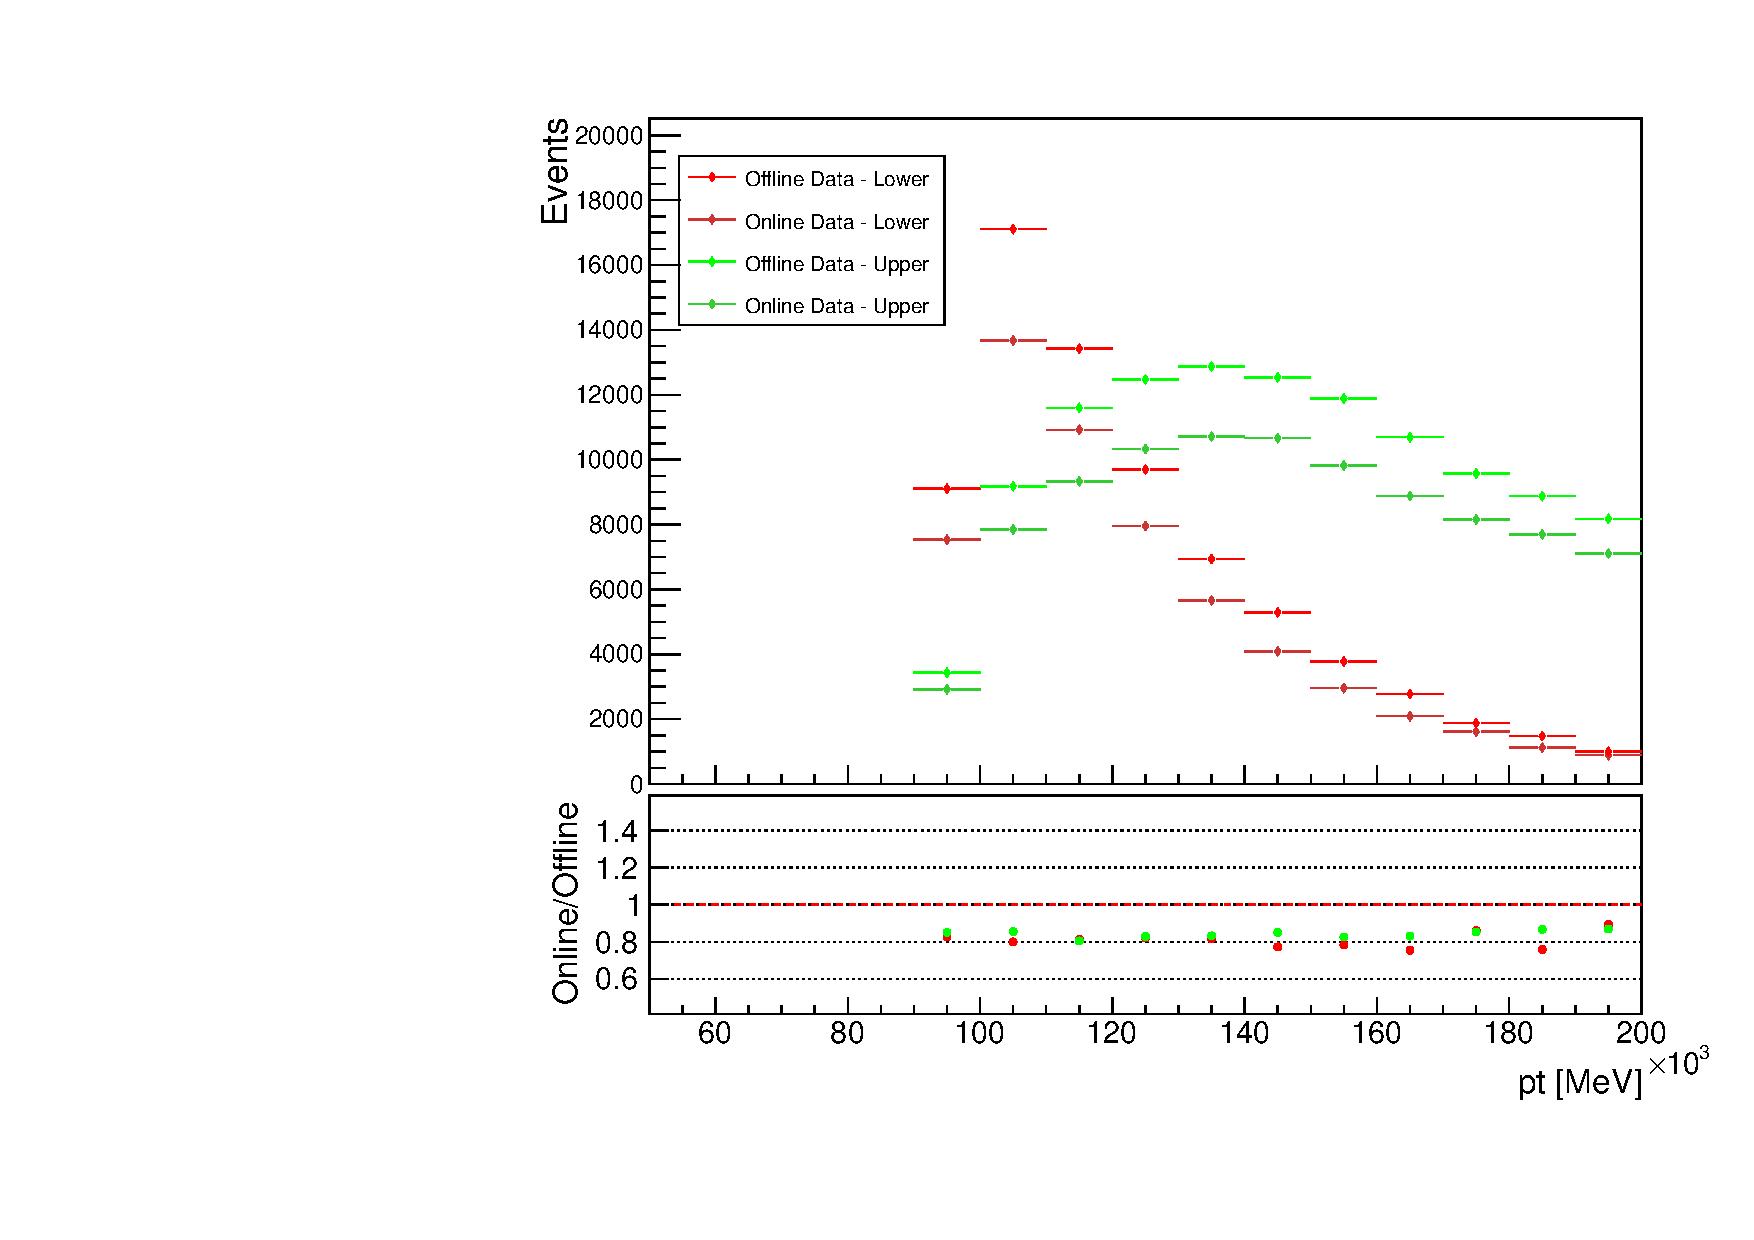
\includegraphics[width=1\linewidth]{pt_bJet1_data_}
			\end{minipage}
			\quad
			\begin{minipage}[h]{0.48\linewidth}
				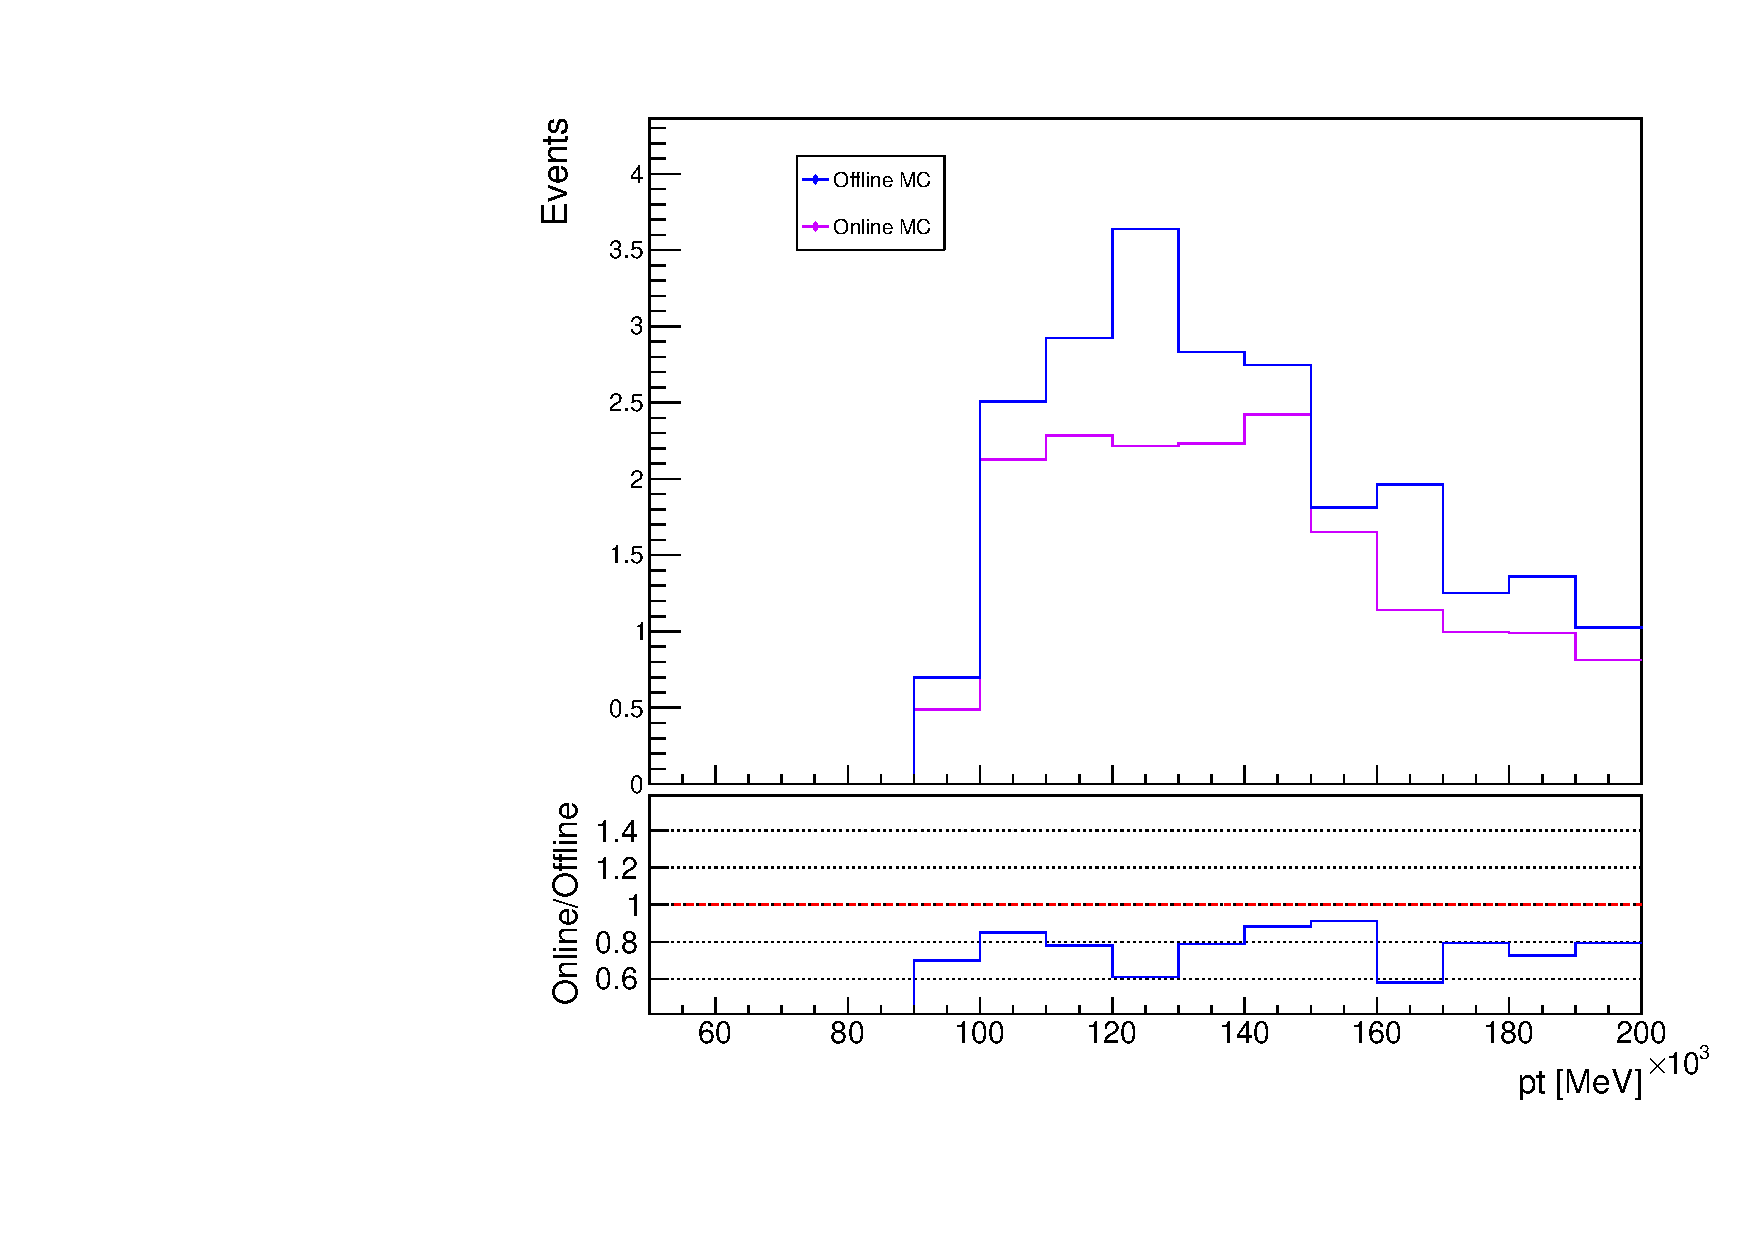
\includegraphics[width=1\linewidth]{pt_bJet1_mc_}
			\end{minipage}
			\label{f:ptb1}
			\caption[\pt distribution of the leading \bjet\ of the \VBFHBB\ event]{\pt distribution of the leading \bjet\ of the \VBFHBB\ event, plotted for both the backgroud data regions in the left panel and Monte-Carlo signal events in the right panel.}
		\end{figure}

	The ratio plot in the left panel of Figure \ref{f:ptb1} shows a flat line in both the upper and lower regions just above $0.8$ for the ratio of the number of online jets with respect to the offline jets, consistent with the decrease in final event count shown in Figure \ref{f:cutflowD}. The Monte-Carlo signal plot in the right panel is noisy but shows the ratio to be $\sim0.8$ across the \pt range, consistent with Figure \ref{f:cutflowMC}. As expected based on the higher \mbb requirement the background events for the Upper region are biased towards higher \pt compared to the lower background region.

		\begin{figure}[h]
			\centering

			\begin{minipage}[h]{0.48\linewidth}
				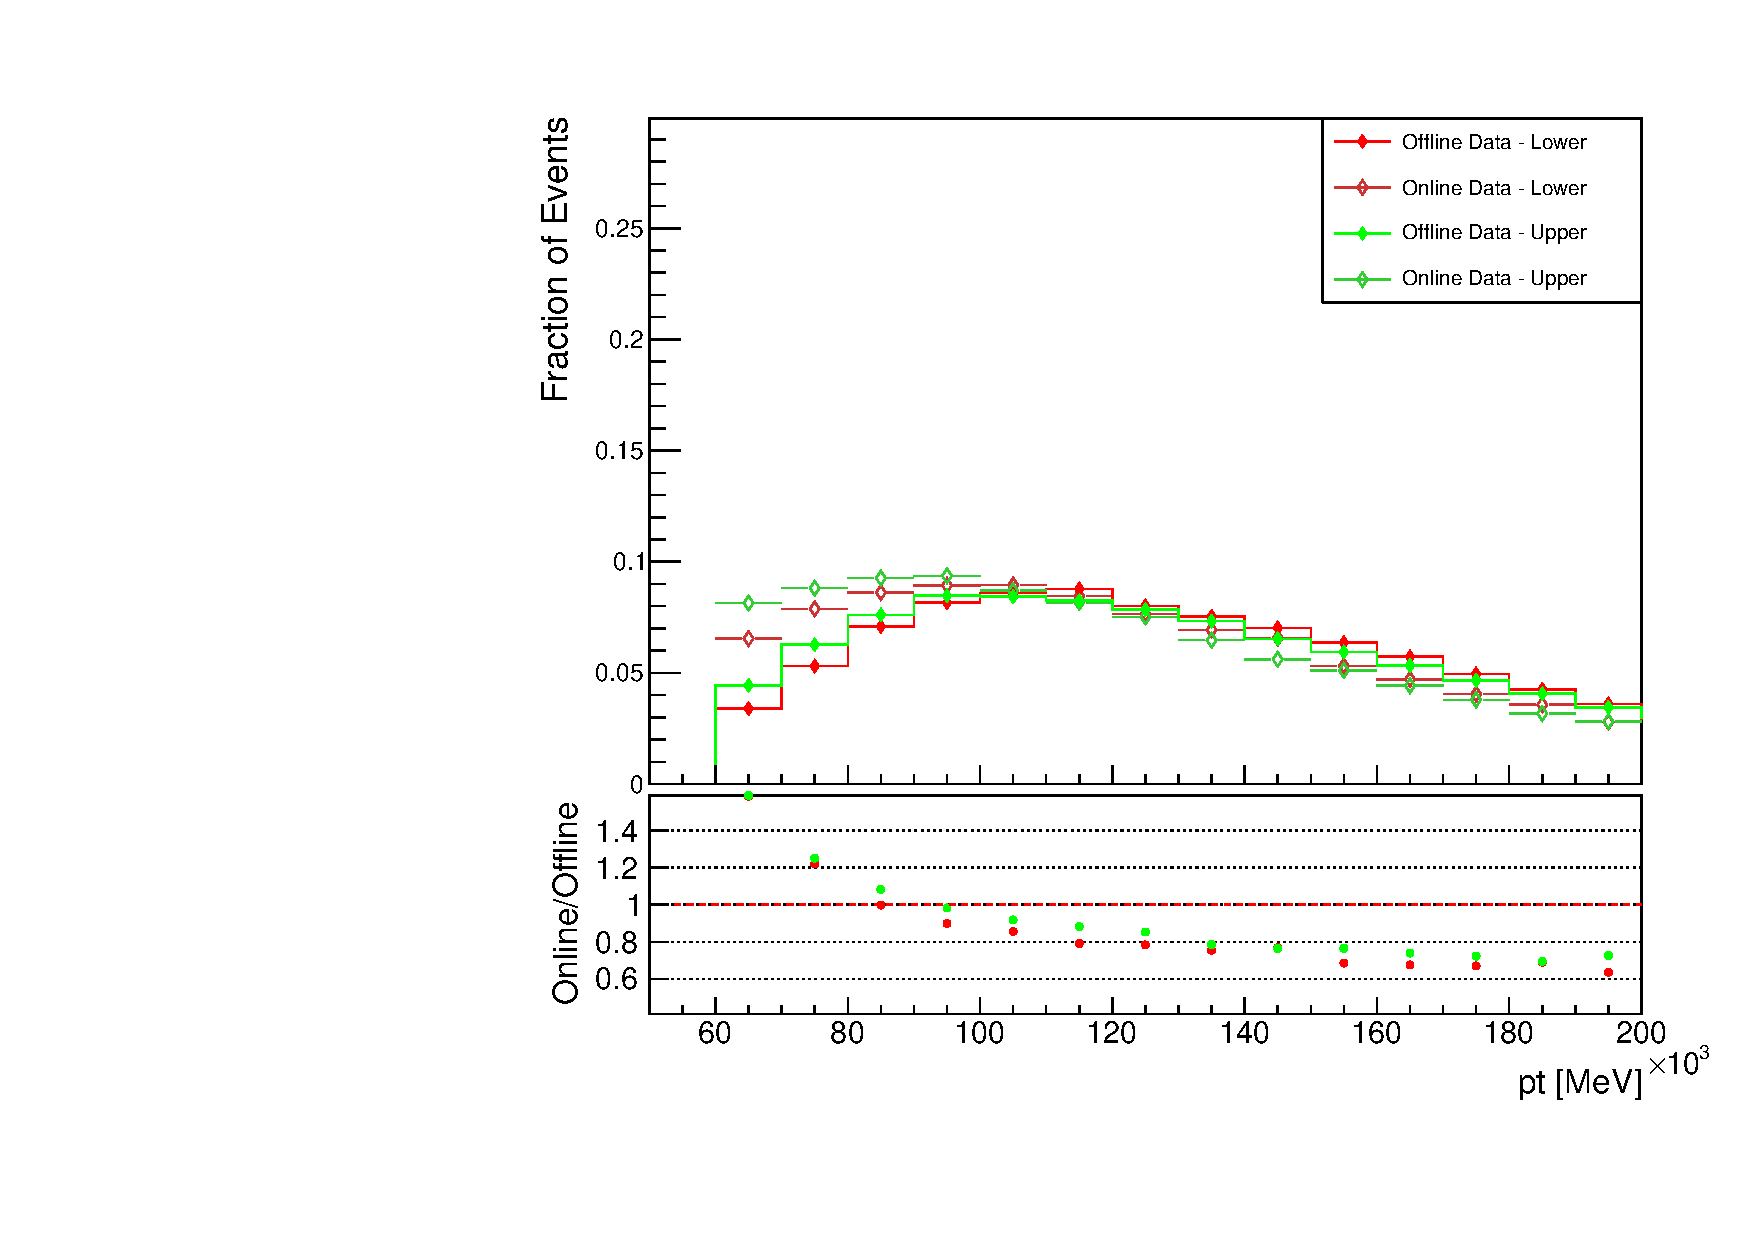
\includegraphics[width=1\linewidth]{pt_lJet1_data_}
			\end{minipage}
			\quad
			\begin{minipage}[h]{0.48\linewidth}
				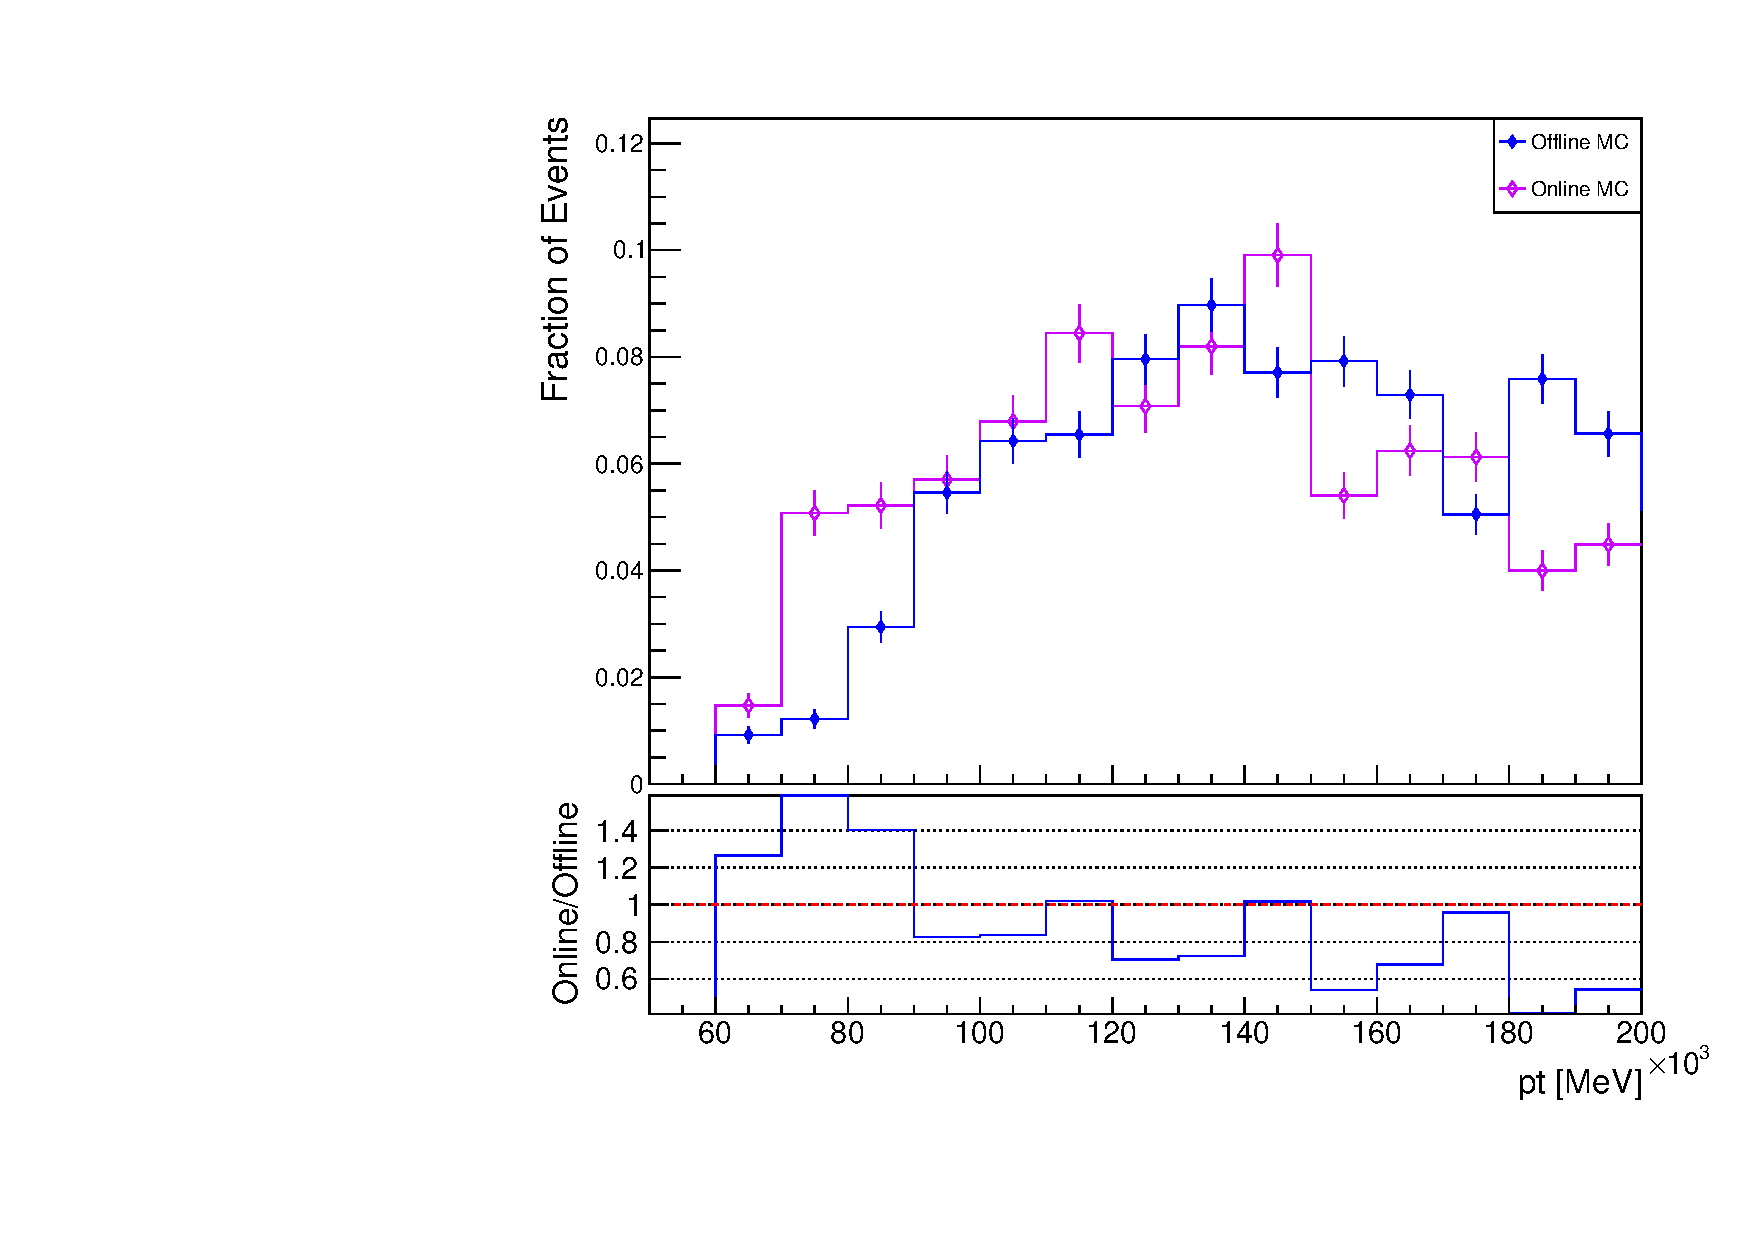
\includegraphics[width=1\linewidth]{pt_lJet1_mc_}
			\end{minipage}
			\label{f:ptj1}
				\caption[\pt distribution of the leading non-\bjet\ of the \VBFHBB\ event]{\pt distribution of the leading non-\bjet\ of the \VBFHBB\ event, plotted for both the backgroud data regions in the left panel and Monte-Carlo signal events in the right panel.}
		\end{figure}

	The relative online and offline behaviour of $j_1$ is slightly more complicated that jet $b_1$. Both the data and Monte-Carlo simulation show a consistent curve in behaviour, with online events being more numerous at low \pt than offline, before the ratio tails off below unity at $\sim90$GeV in both the plots in Figure \ref{f:ptj1} to $\sim 0.7$ in the data. The Monte-Carlo plot jumps around, but the comparitive online/offline performance trends in the same fashion as the background plot.

		\begin{figure}[h]
			\centering

			\begin{minipage}[h]{0.48\linewidth}
				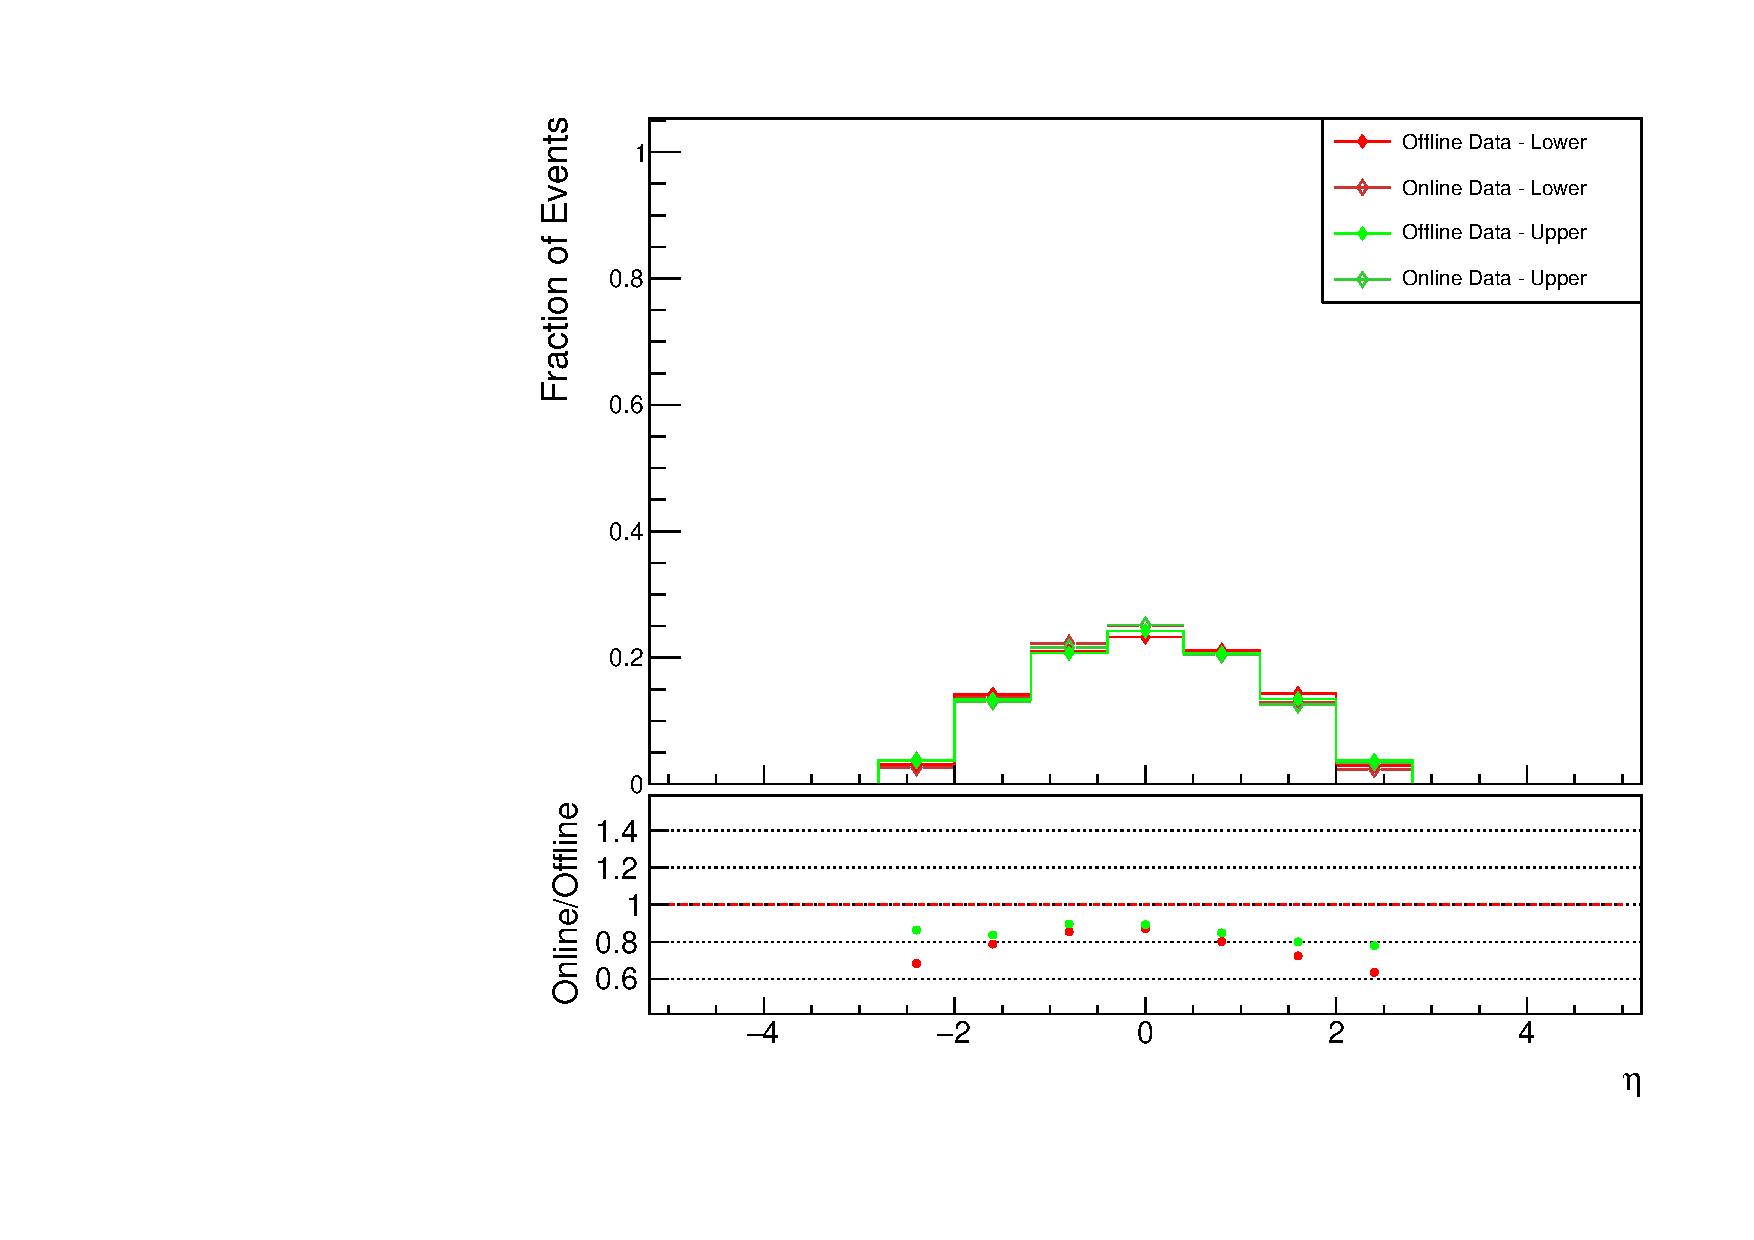
\includegraphics[width=1\linewidth]{eta_bJet1_data_}
			\end{minipage}
			\quad
			\begin{minipage}[h]{0.48\linewidth}
				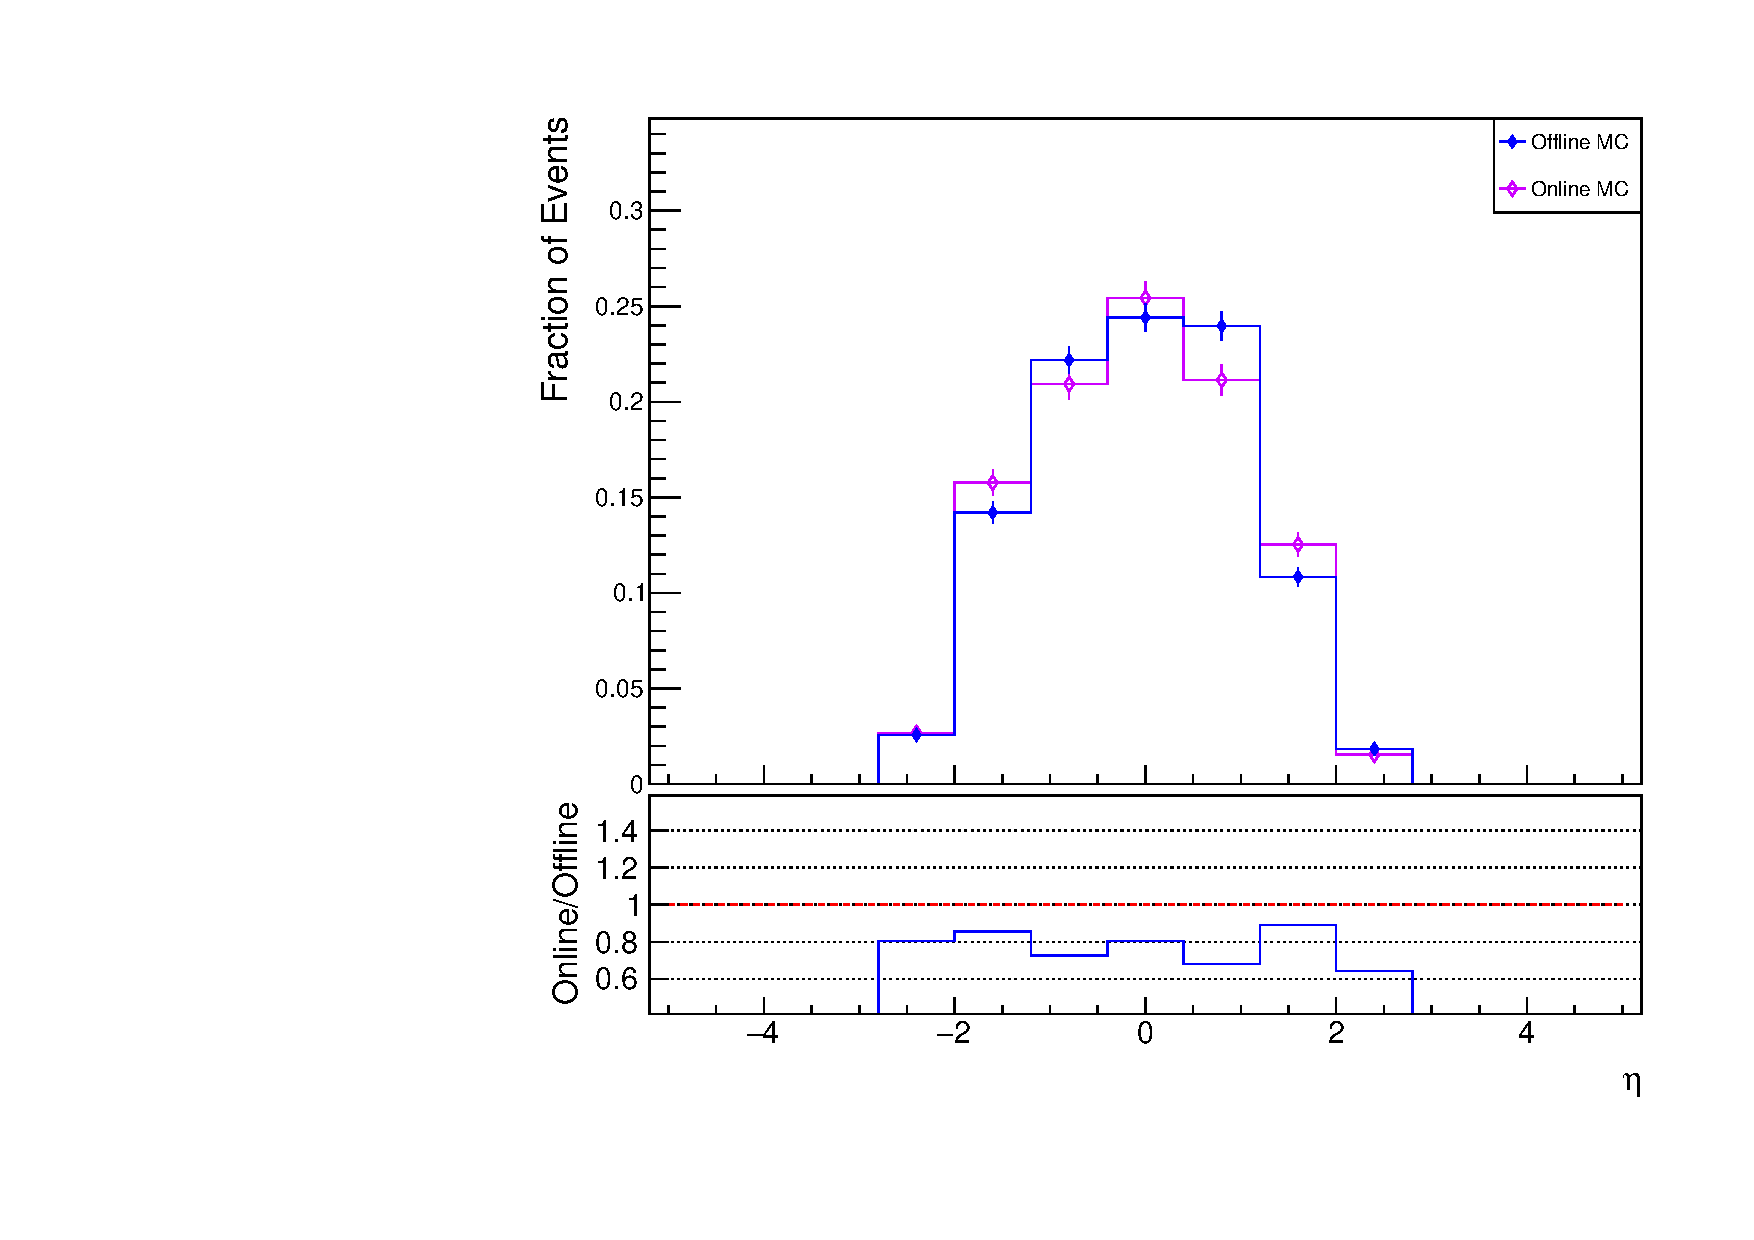
\includegraphics[width=1\linewidth]{eta_bJet1_mc_}
			\end{minipage}
			\label{f:etab1}
			\caption[$\eta$ distribution of the leading \bjet\ of the \VBFHBB\ event]{$\eta$ distribution of the leading \bjet\ of the \VBFHBB\ event, plotted for both the backgroud data regions in the left panel and Monte-Carlo signal events in the right panel.}
		\end{figure}

	Figure \ref{f:etab1} shows shared distribution shapes between the online and offline objects for both signal and background, and the consistency of the online distribution against the offline is also shown for the leading non-\bjet\ in Figure \ref{f:etaj1}. The data distribution for $b_1$ in the left panel of Figure \ref{f:etab1} shows a pronounced curve in the online and offline ratio, with more online events surviving the cuts in the central regions, and the overall efficiency being roughly consistent with the expected $\sim0.8$ value. The signal distribution in the right panel shows a flatter ratio distribution, also around this value.

		\begin{figure}[h]
			\centering
			\begin{minipage}[h]{0.48\linewidth}
				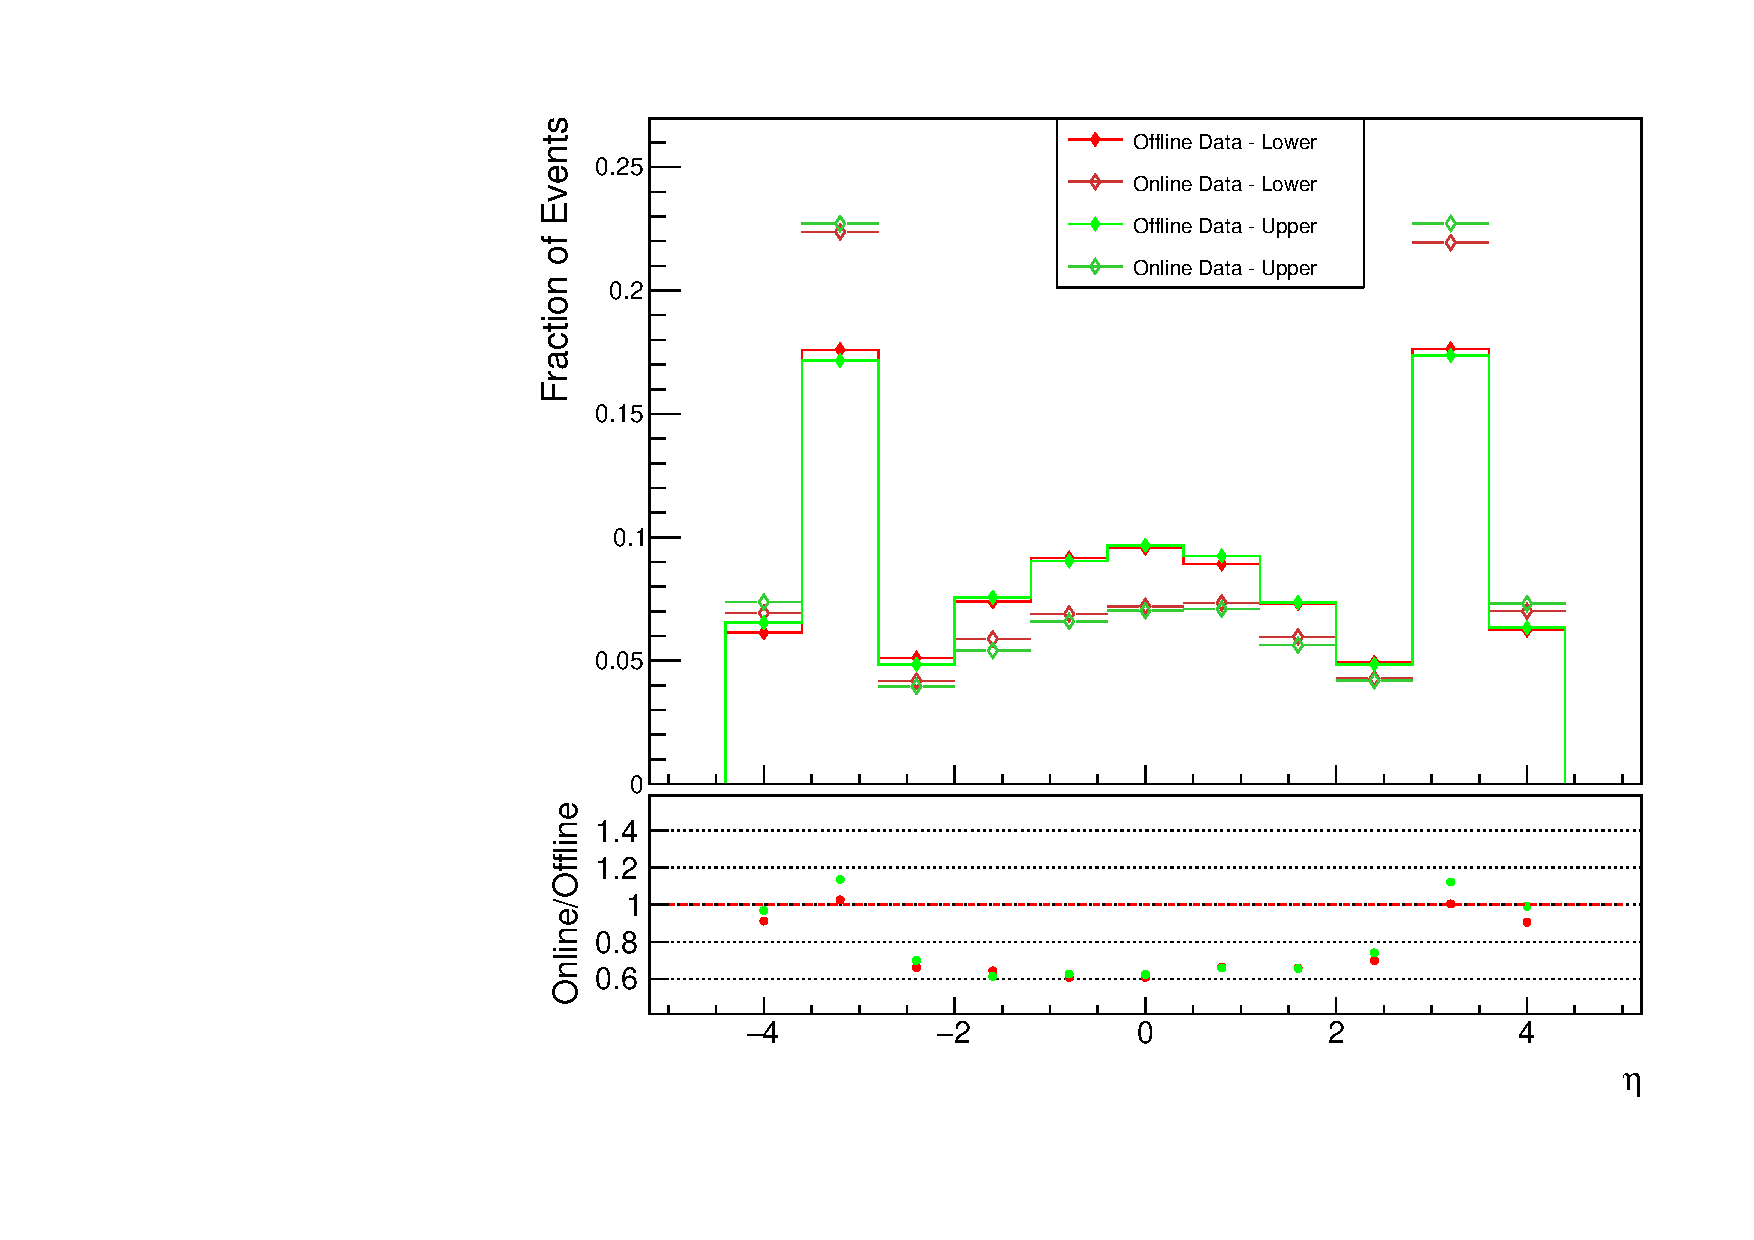
\includegraphics[width=1\linewidth]{eta_lJet1_data_}
			\end{minipage}
			\quad
			\begin{minipage}[h]{0.48\linewidth}
				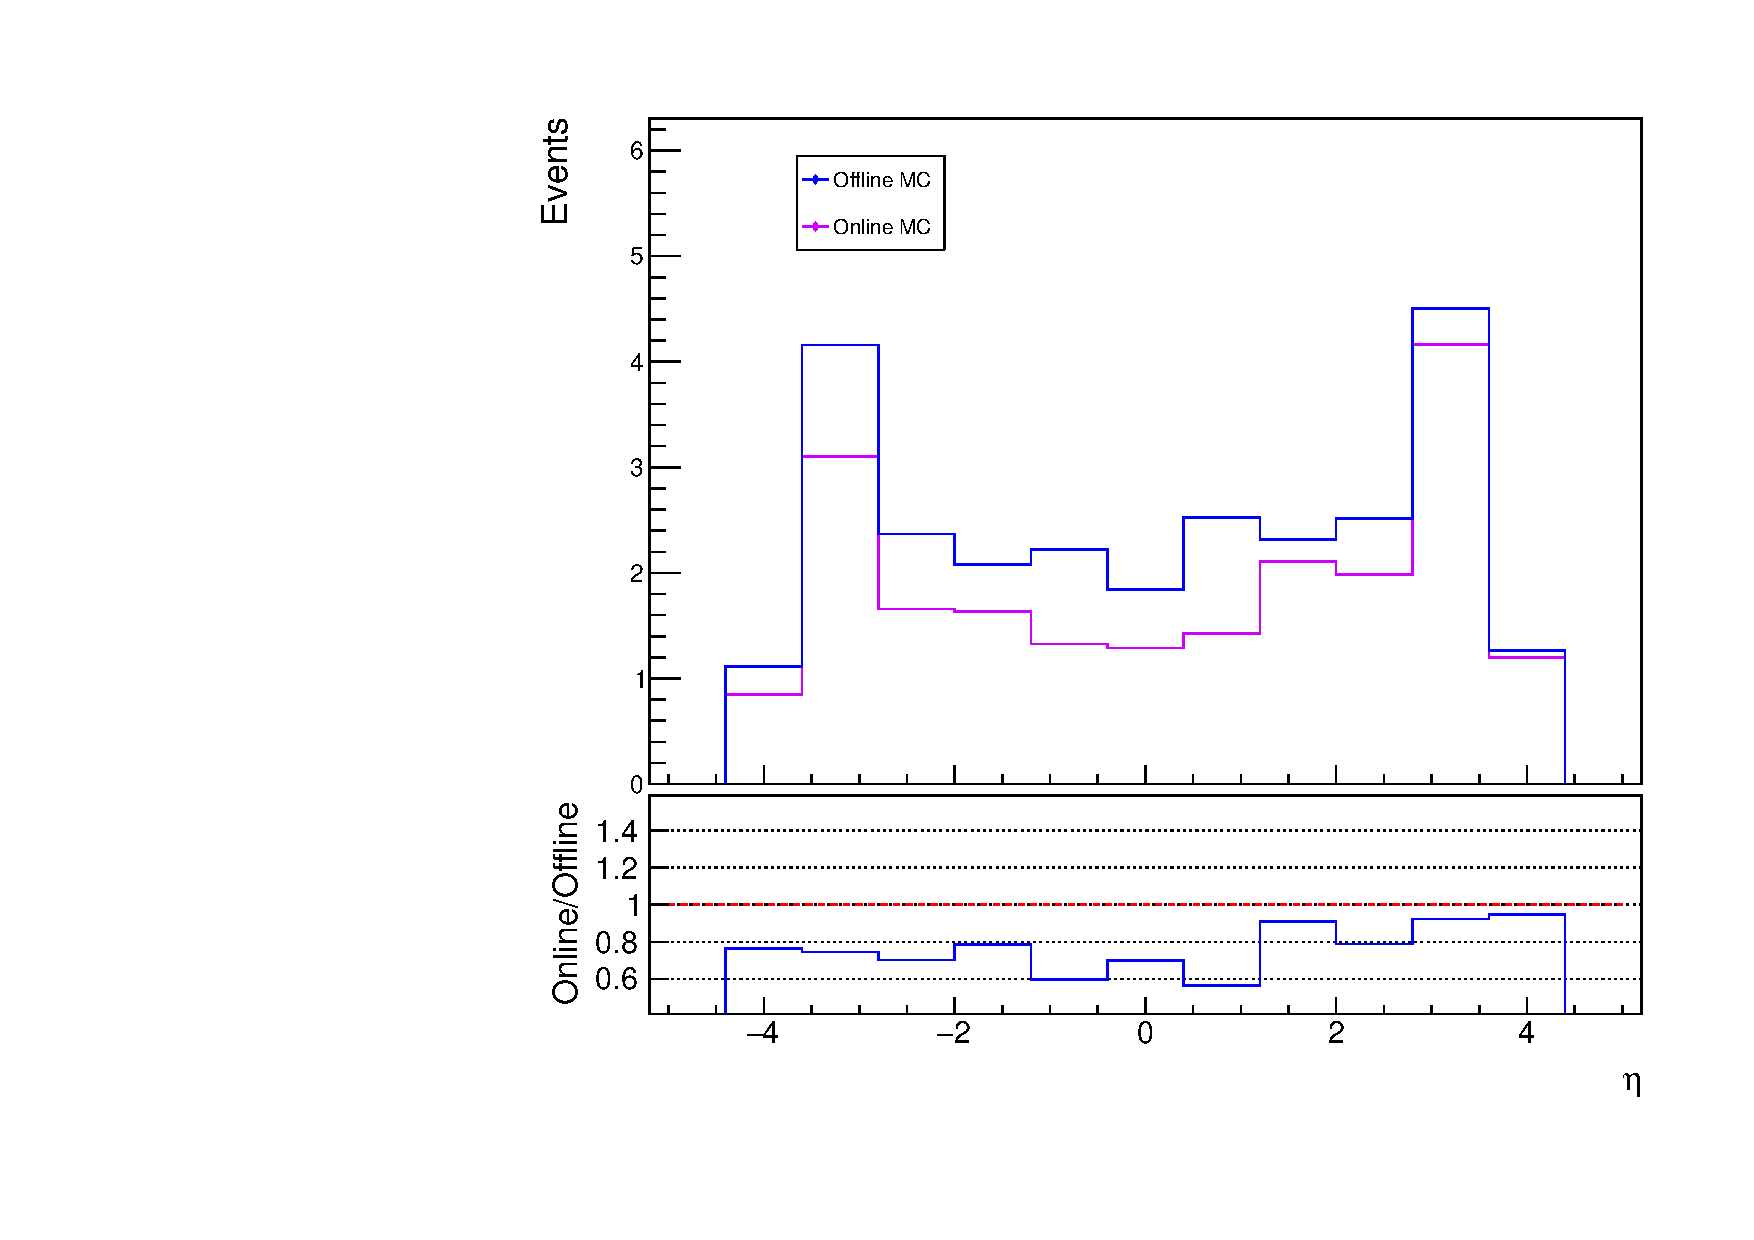
\includegraphics[width=1\linewidth]{eta_lJet1_mc_}
			\end{minipage}
			\label{f:etaj1}
			\caption[$\eta$ distribution of the leading non-\bjet\ of the \VBFHBB\ event]{$\eta$ distribution of the leading non-\bjet\ of the \VBFHBB\ event, plotted for both the backgroud data regions in the left panel and Monte-Carlo signal events in the right panel.}
		\end{figure}

		The $\eta$ distribution for the leading non-\bjet\ shows spikes in  forward region  both the background and signal plots in Figure \ref{f:etaj1}, which is expected given the jet criteria required for a \VBFHBB\ event. Both plots show the decrease in the online events relative to the offline events expected in each of these.

	\subsection{Summary of the \VBFHBB\ jet objects}

	The plots for the \VBFHBB\ final state mostly show agreement, with respect to the overall decrease in the event rate for online events, between the online and offline distributions of the kinematic quantities of the jets for signal and background. The shapes if the distributions are consistent between the background and signal events, and the specific features like the forward jet spikes in Figure \ref{f:etaj1} and the increase \pt of the upper background sector in Figure \ref{f:ptb1} are explainable by considering the topology of a \VBFHBB\ event.

	There are two sections of these plots where the online/offline comparison significantly deviates from the demonstrated efficiency of $\sim80\%$, in Figure \ref{f:ptj1} for low \pt non-\bjets and in Figure \ref{f:etaj1} for the high $\eta$ non-\bjets. Both these artifacts could be a result of additional forward jets in the online events. A forward jet compared to a jet with identical momentum jet at a central eta will have a lower \pt given the geometry of the jet and the definition of \pt.

	An additional difference was the upper background sector frequently had a higher ratio than the lower background sector, as shown across the entire \pt range in Figures \ref{f:ptb1} and \ref{f:ptj1}.
}

\section{Kinematic quantities of the \VBFHBB\ event}

		\begin{figure}[h]
			\centering
			\begin{minipage}[h]{0.48\linewidth}
				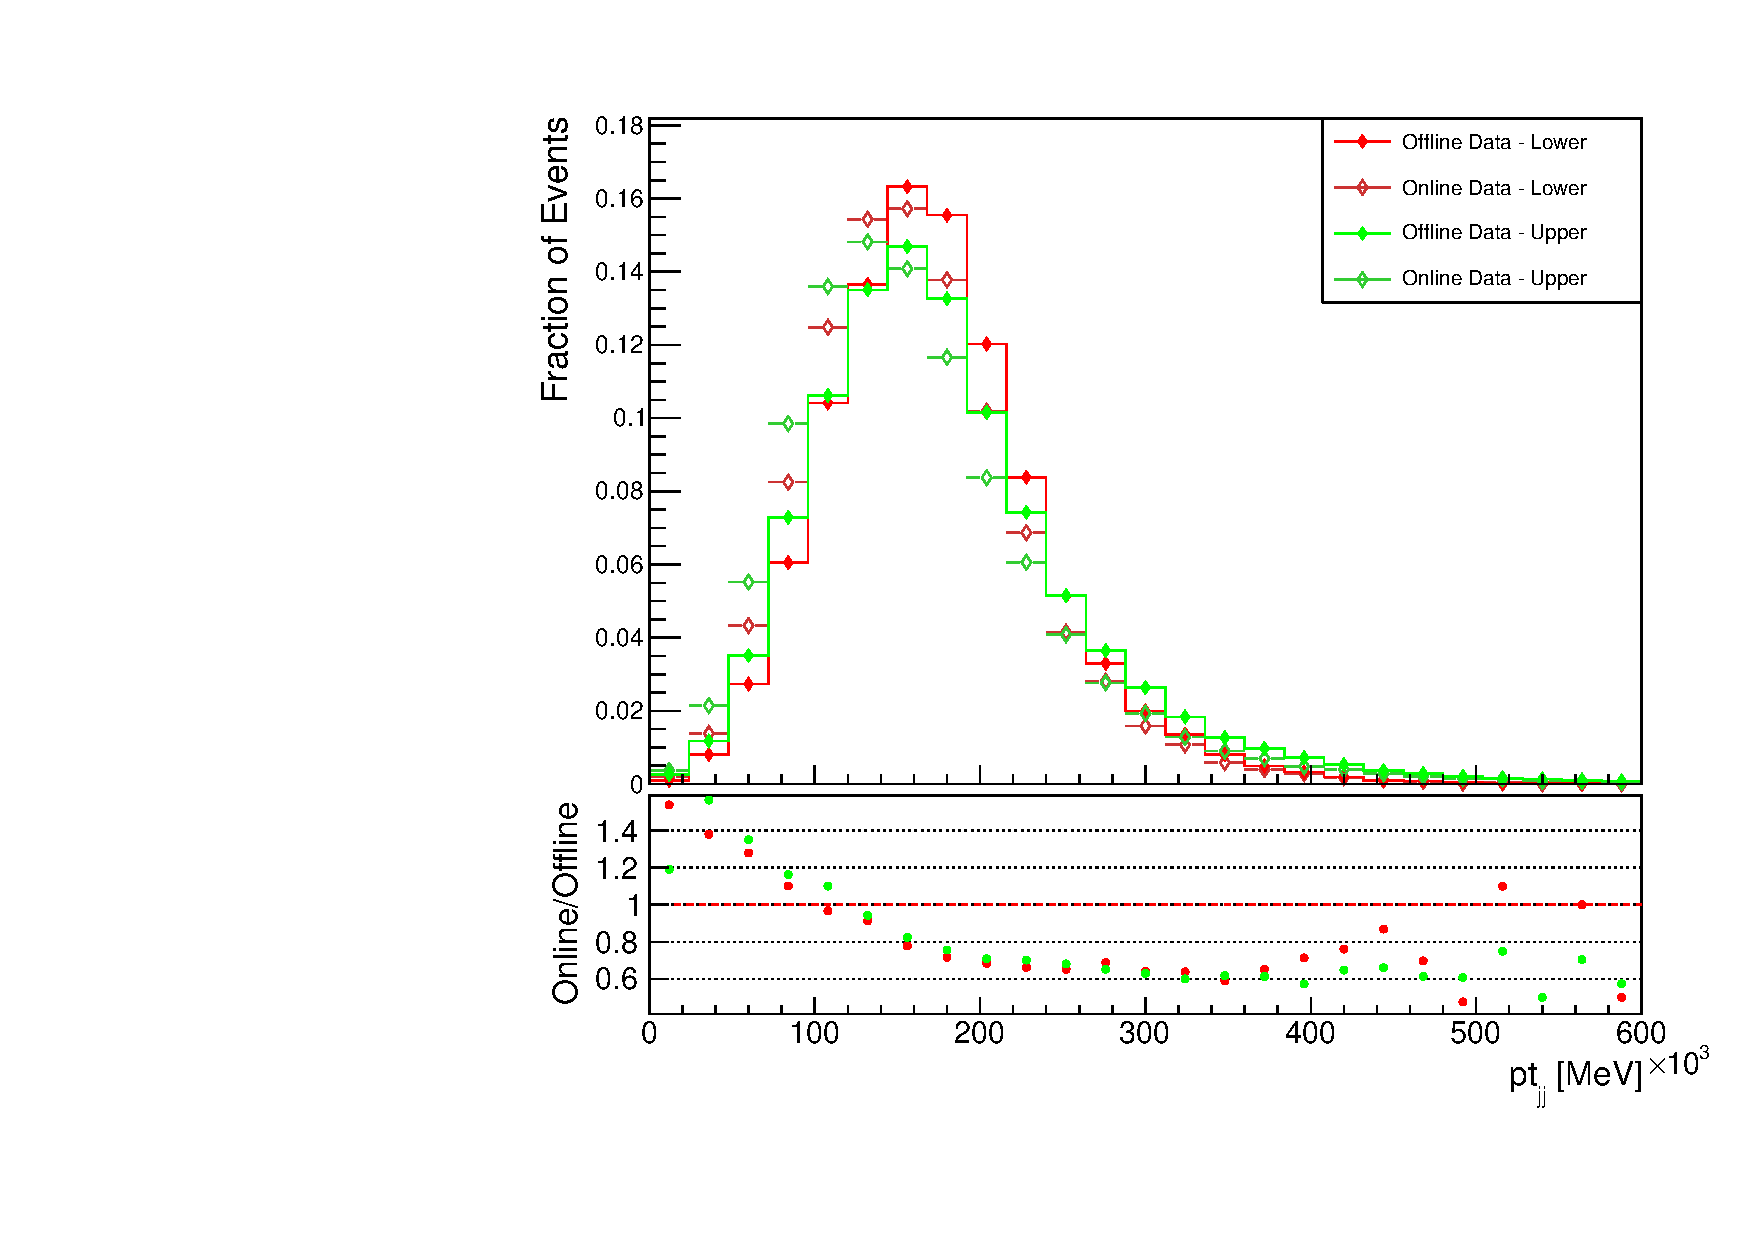
\includegraphics[width=1\linewidth]{ptjj_data_}
			\end{minipage}
			\quad
			\begin{minipage}[h]{0.48\linewidth}
				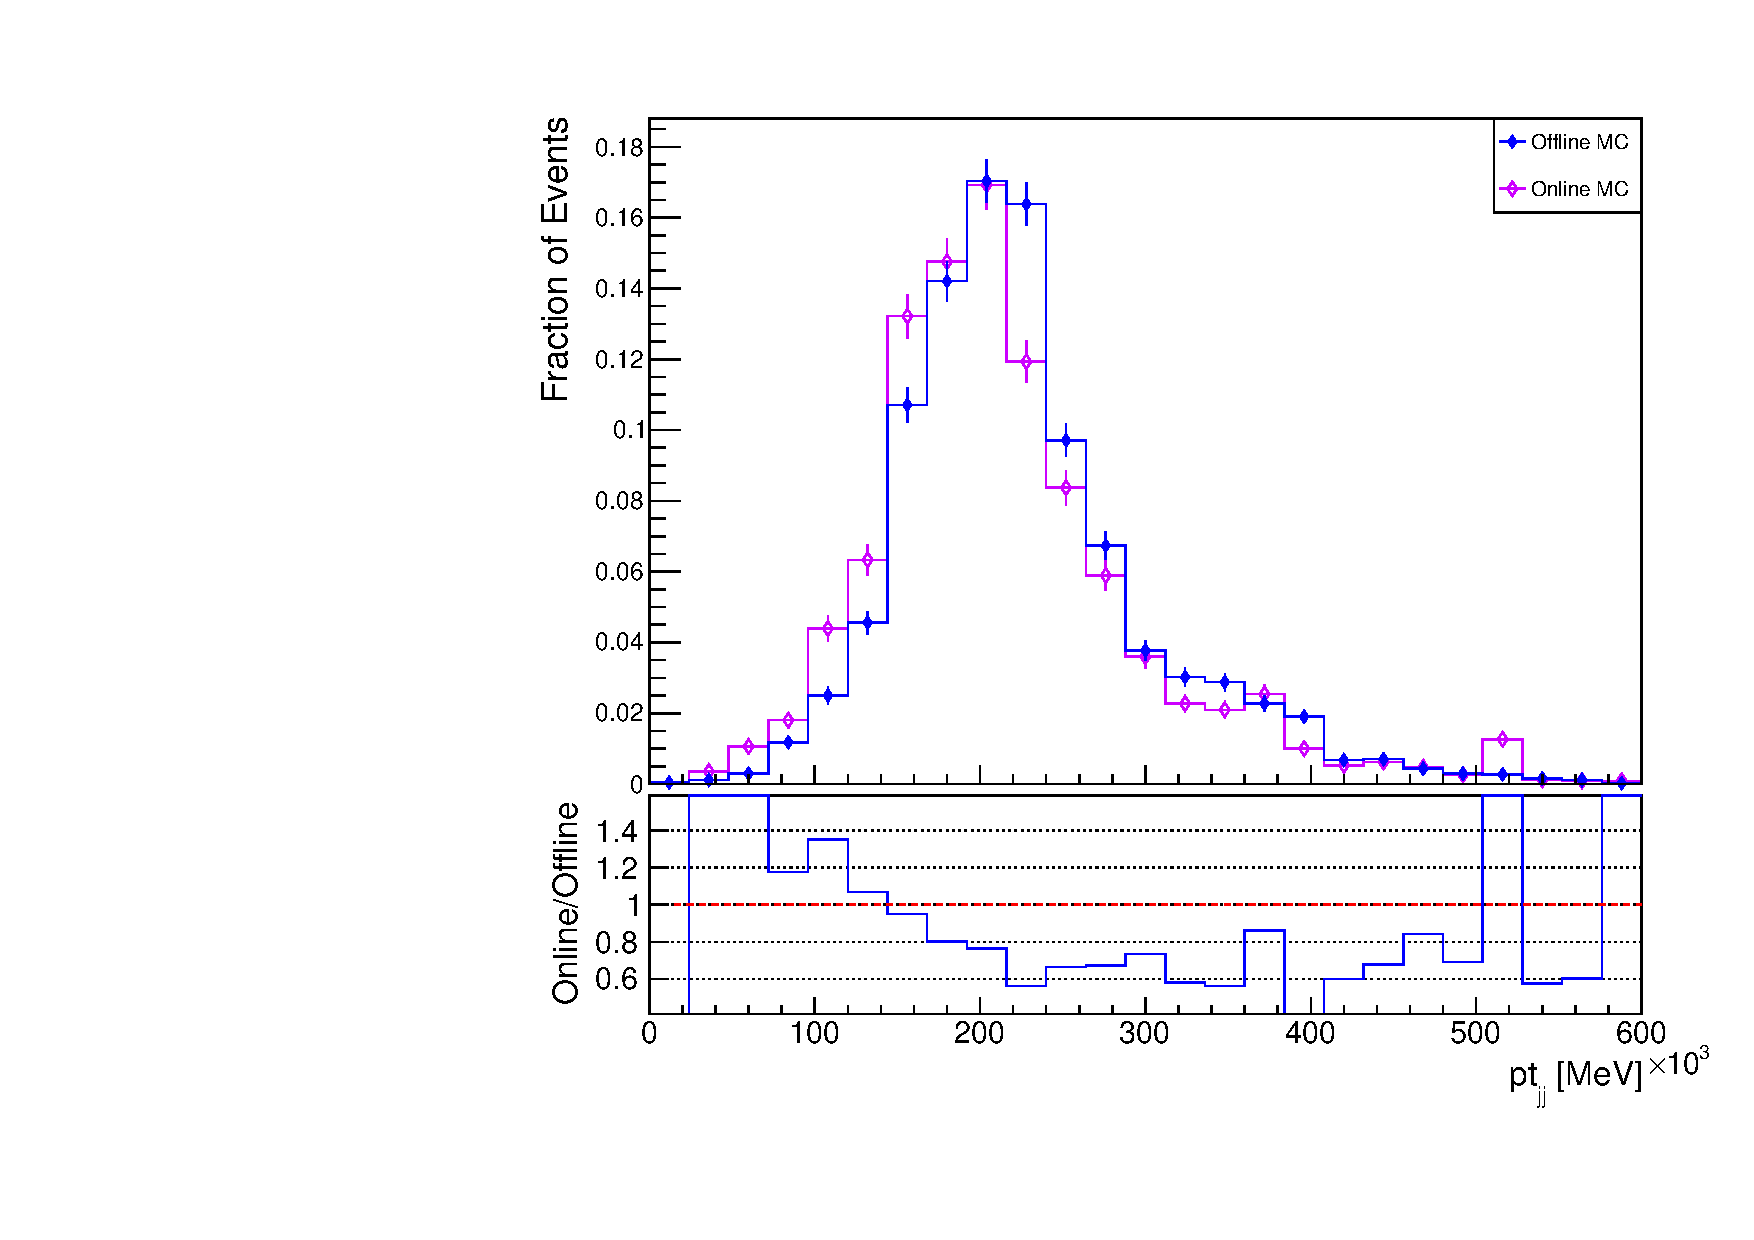
\includegraphics[width=1\linewidth]{ptjj_mc_}
			\end{minipage}
			\label{f:ptjj}
			\caption[Comparison of the \ptjj distribution of the \VBFHBB\ events for HLT and offline objects]{\ptjj distribution for the online and offline \VBFHBB\ events, with background events from data shown in the left panel and Monte-Carlo signal events in the right.}
		\end{figure}

		\begin{figure}[h]
			\centering
			\begin{minipage}[h]{0.48\linewidth}
				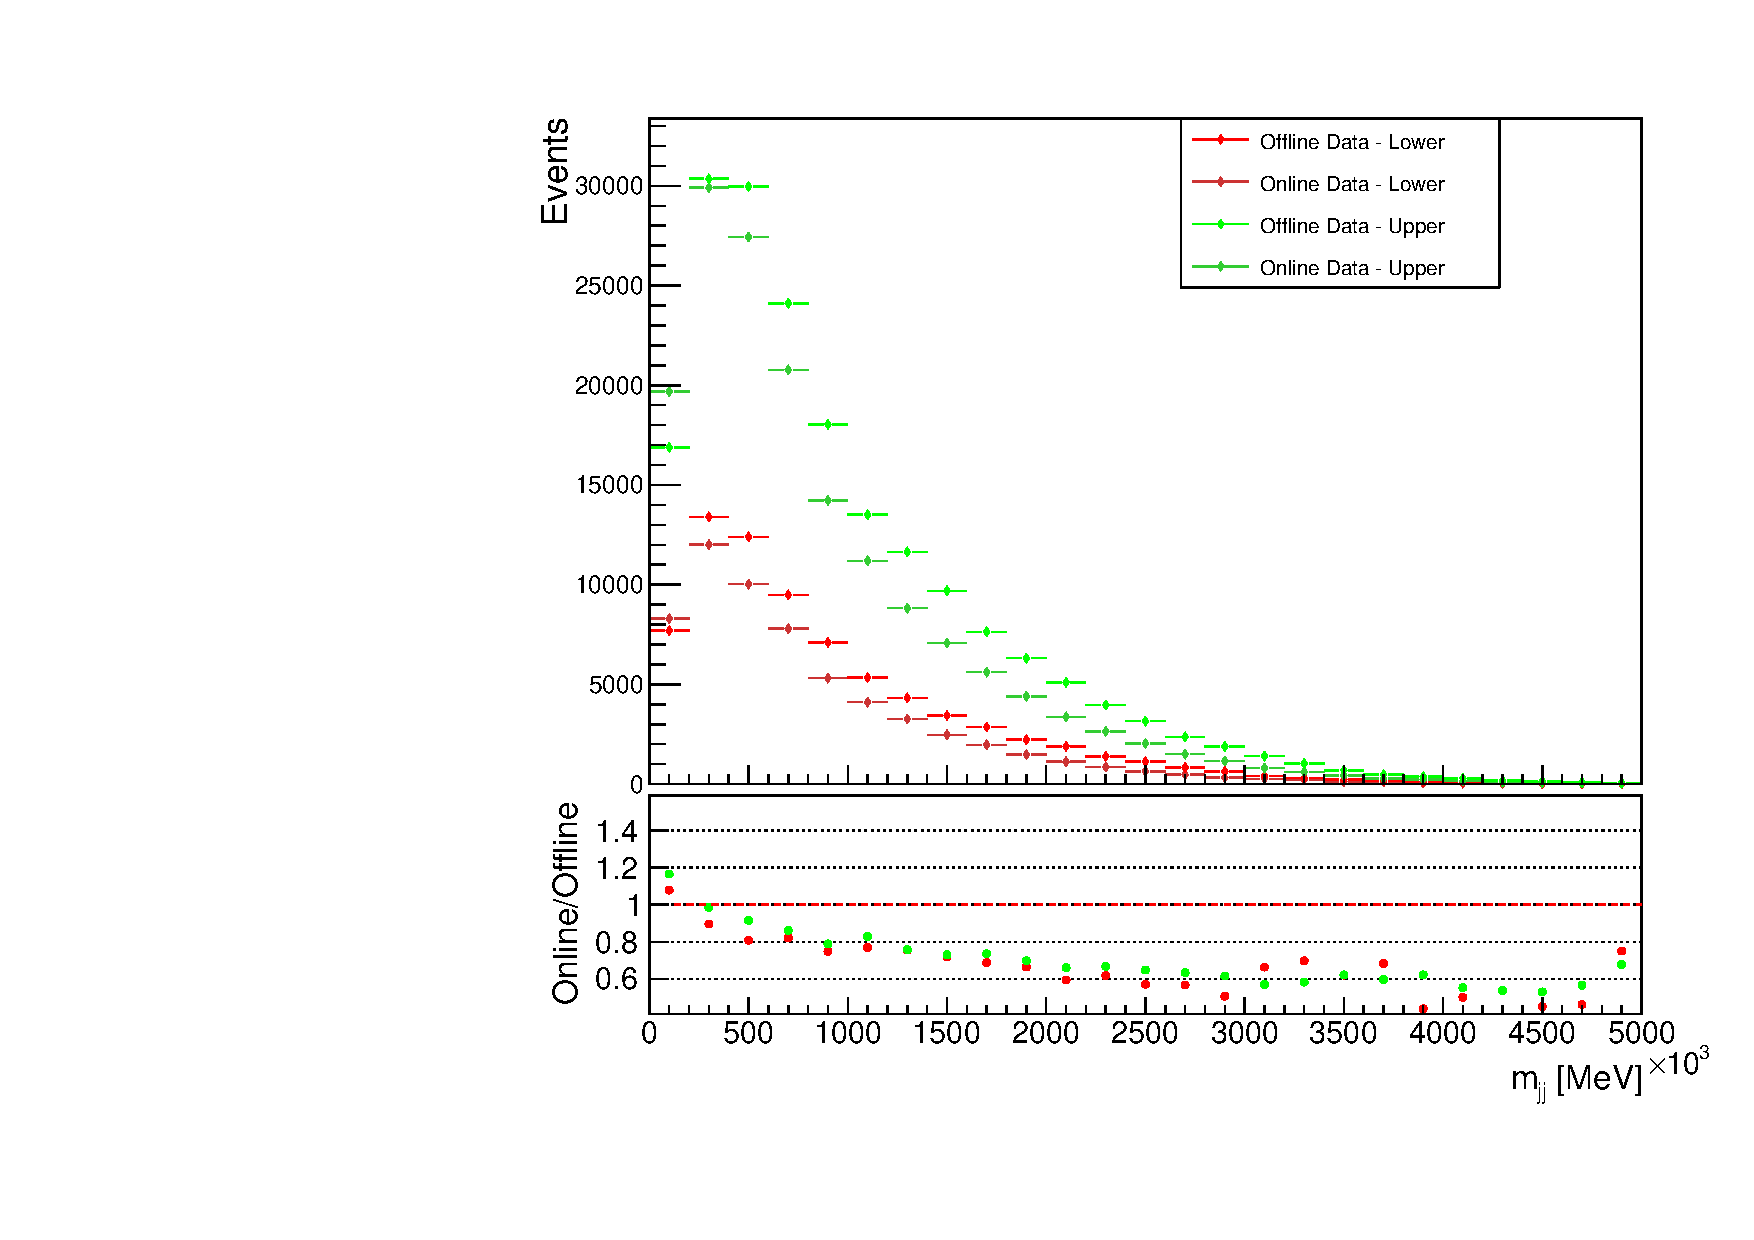
\includegraphics[width=1\linewidth]{mjj_data_}
			\end{minipage}
			\quad
			\begin{minipage}[h]{0.48\linewidth}
				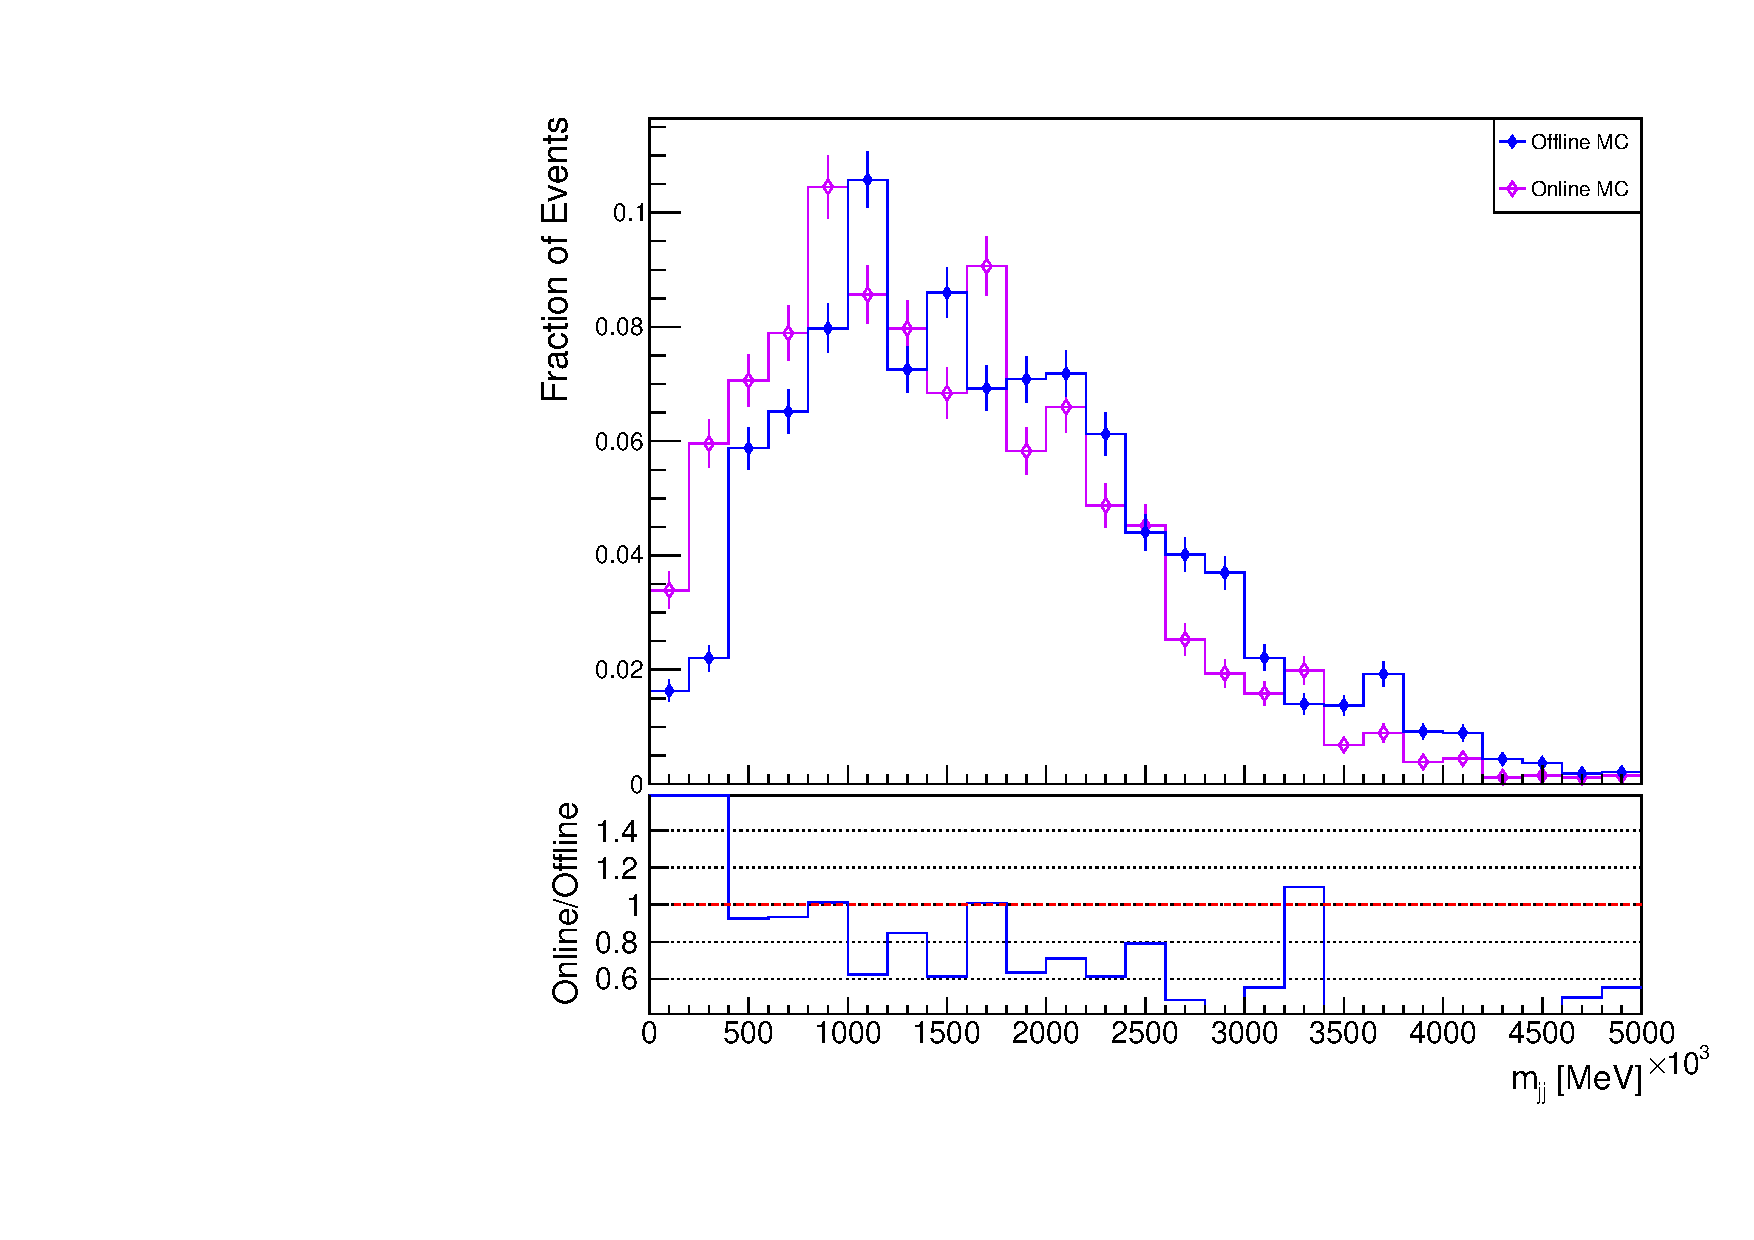
\includegraphics[width=1\linewidth]{mjj_mc_}
			\end{minipage}
			\label{f:mjj}
			\caption[Comparison of the \mjj distribution of the \VBFHBB\ events for HLT and offline objects]{\mjj distribution for the online and offline \VBFHBB\ events, with background events from data shown in the left panel and Monte-Carlo signal events in the right.}
		\end{figure}


		\begin{figure}[h]
			\centering
			\begin{minipage}[h]{0.48\linewidth}
				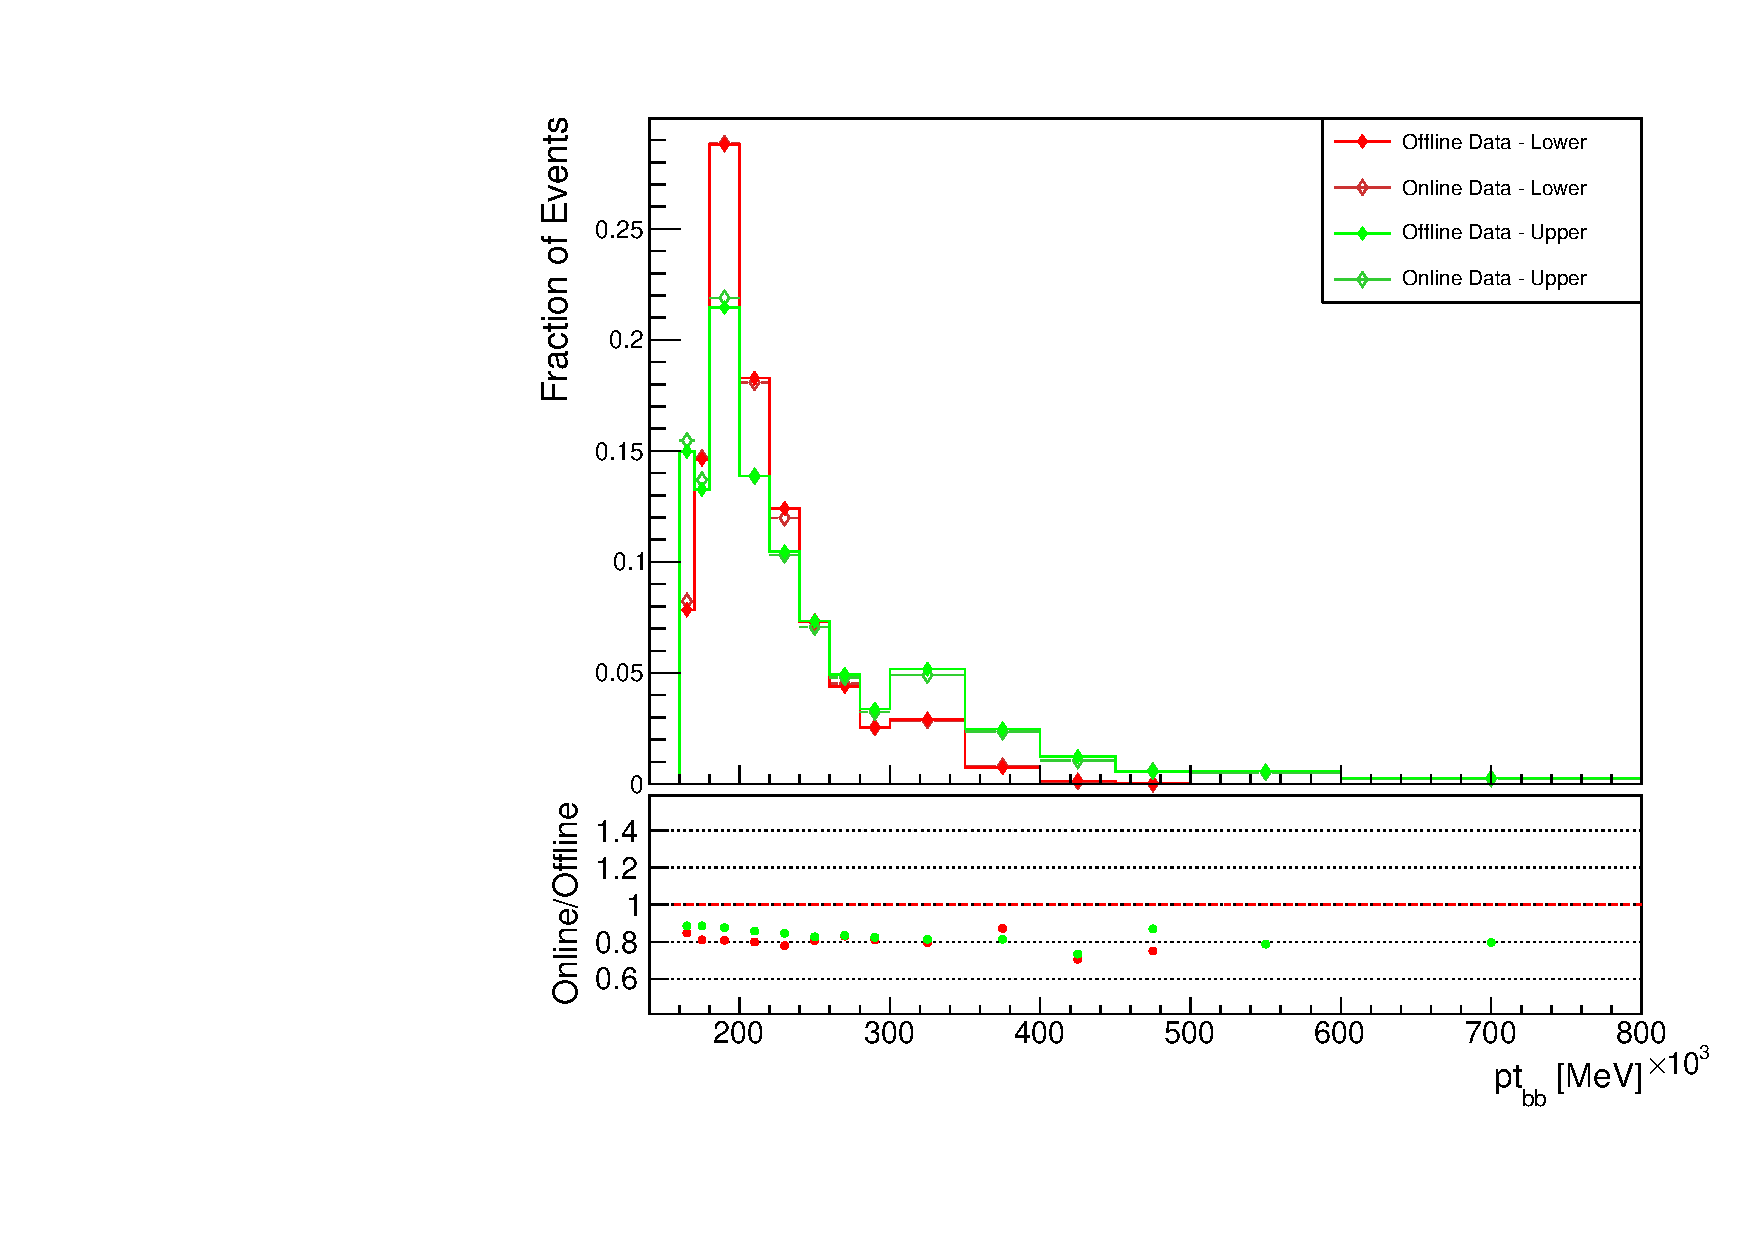
\includegraphics[width=1\linewidth]{ptbb_data_}
			\end{minipage}
			\quad
			\begin{minipage}[h]{0.48\linewidth}
				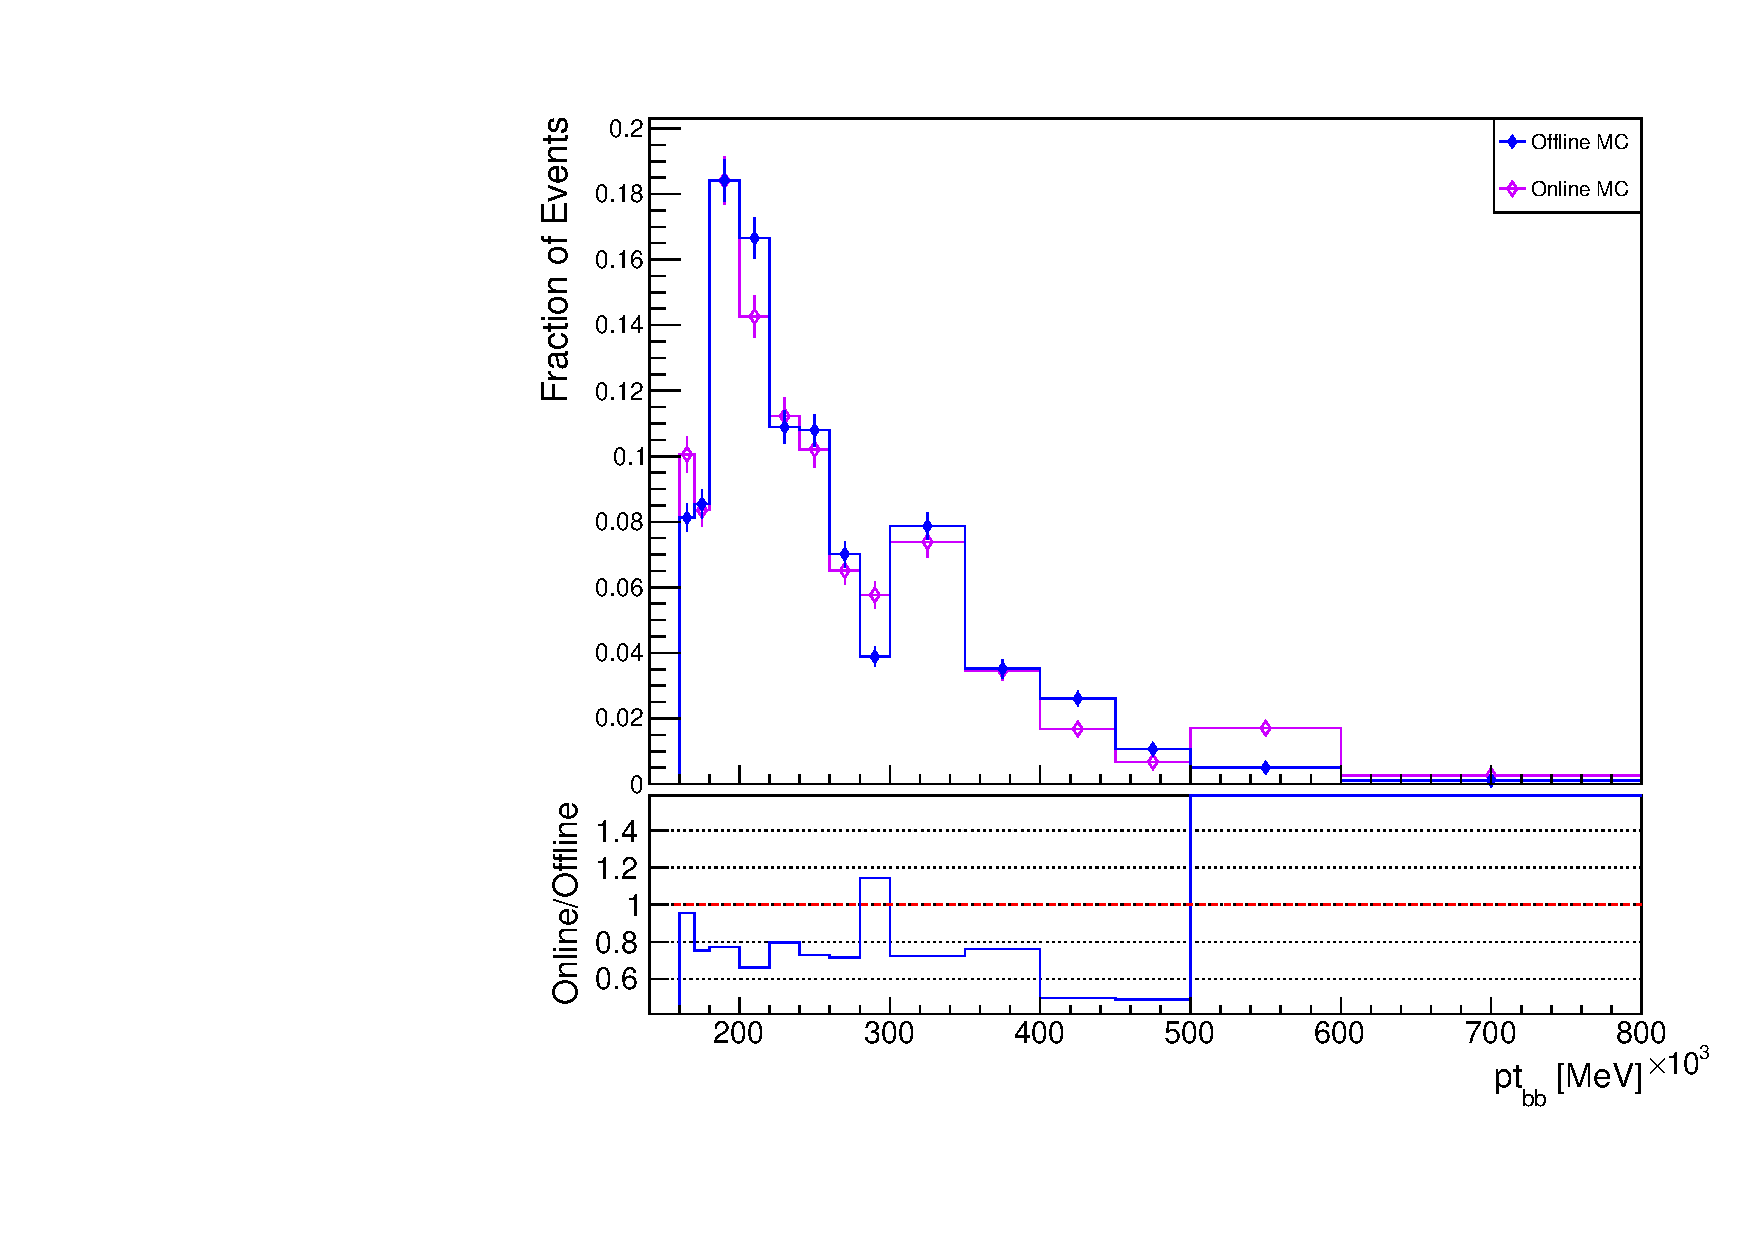
\includegraphics[width=1\linewidth]{ptbb_mc_}
			\end{minipage}
			\label{f:ptbb}
			\caption[Comparison of the \ptbb distribution of the \VBFHBB\ events for HLT and offline objects]{\ptbb distribution for the online and offline \VBFHBB\ events, with background events from data shown in the left panel and Monte-Carlo signal events in the right.}
		\end{figure}

		\begin{figure}[h]
			\centering
			\begin{minipage}[h]{0.48\linewidth}
				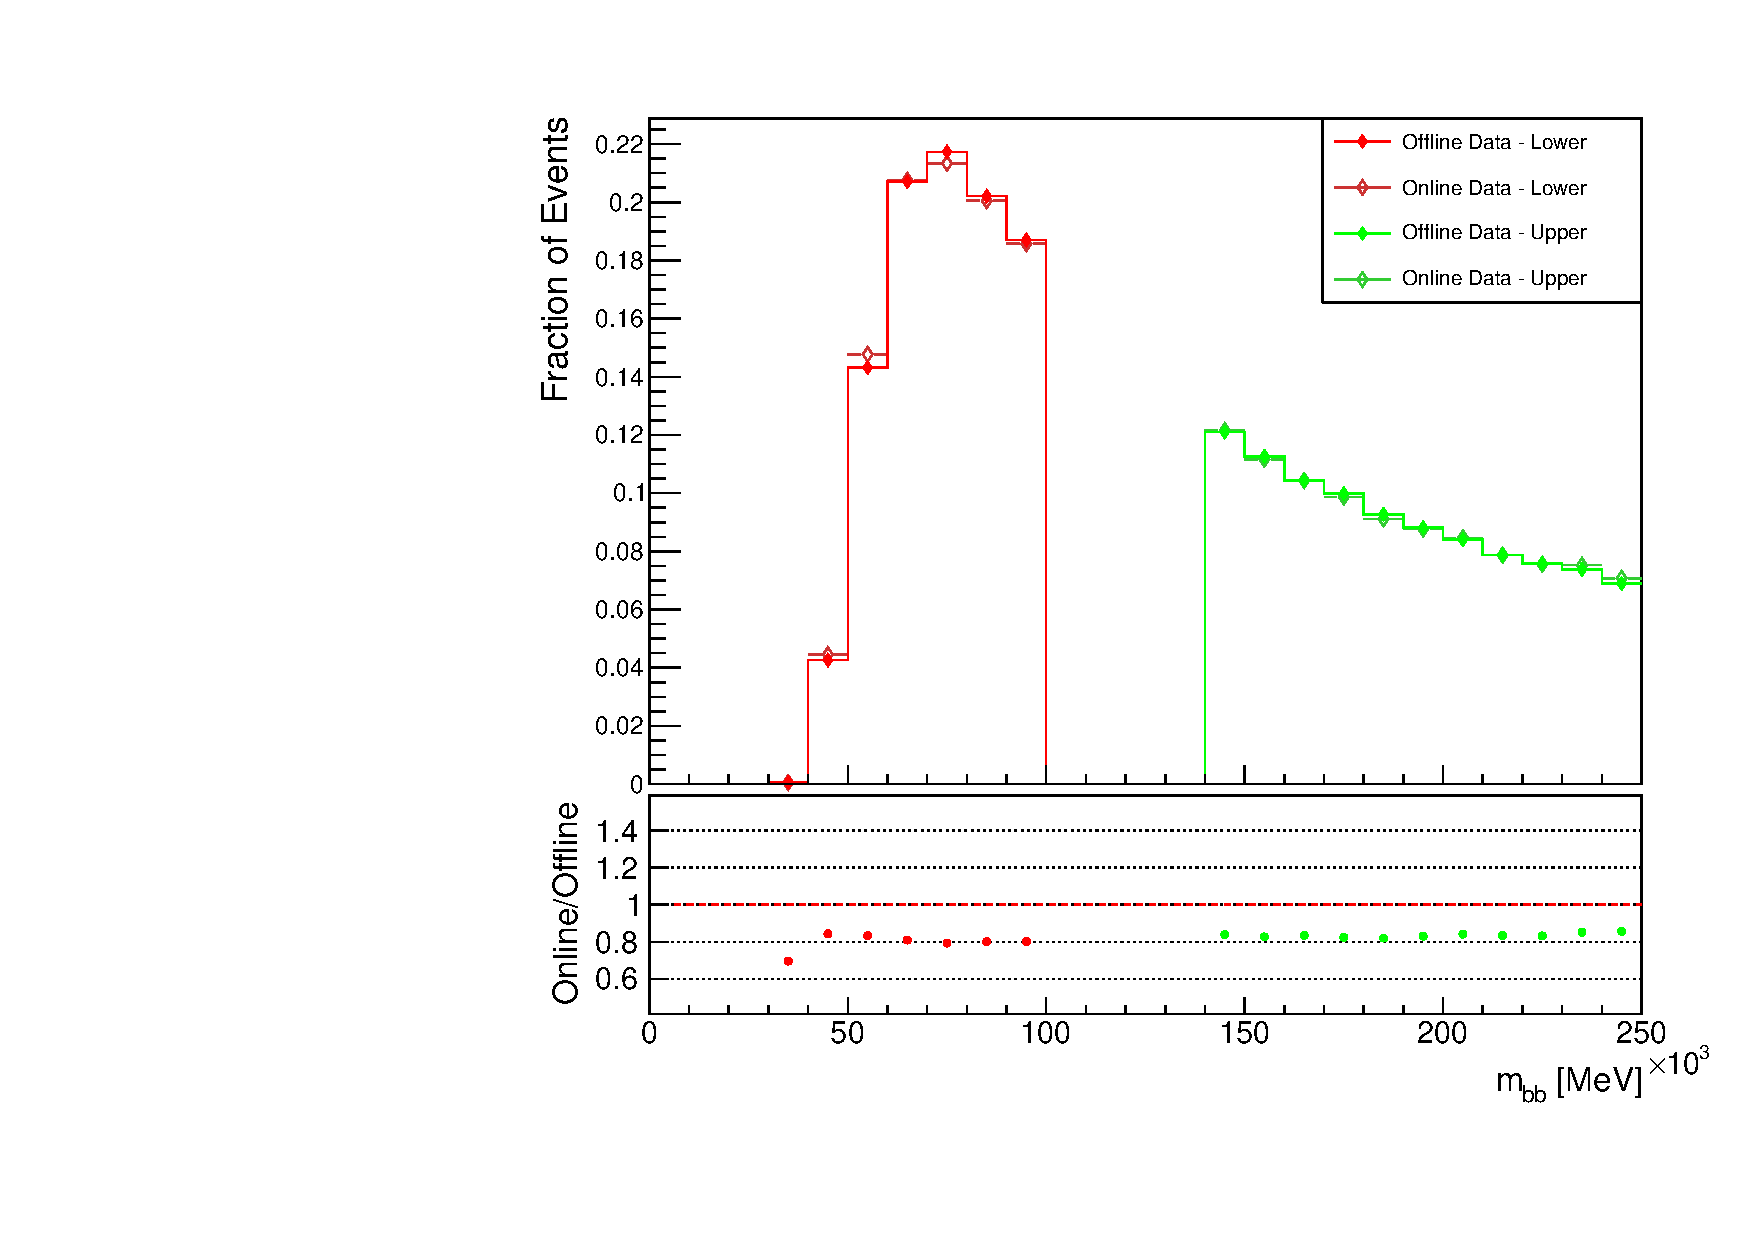
\includegraphics[width=1\linewidth]{mbb_data_}
			\end{minipage}
			\quad
			\begin{minipage}[h]{0.48\linewidth}
				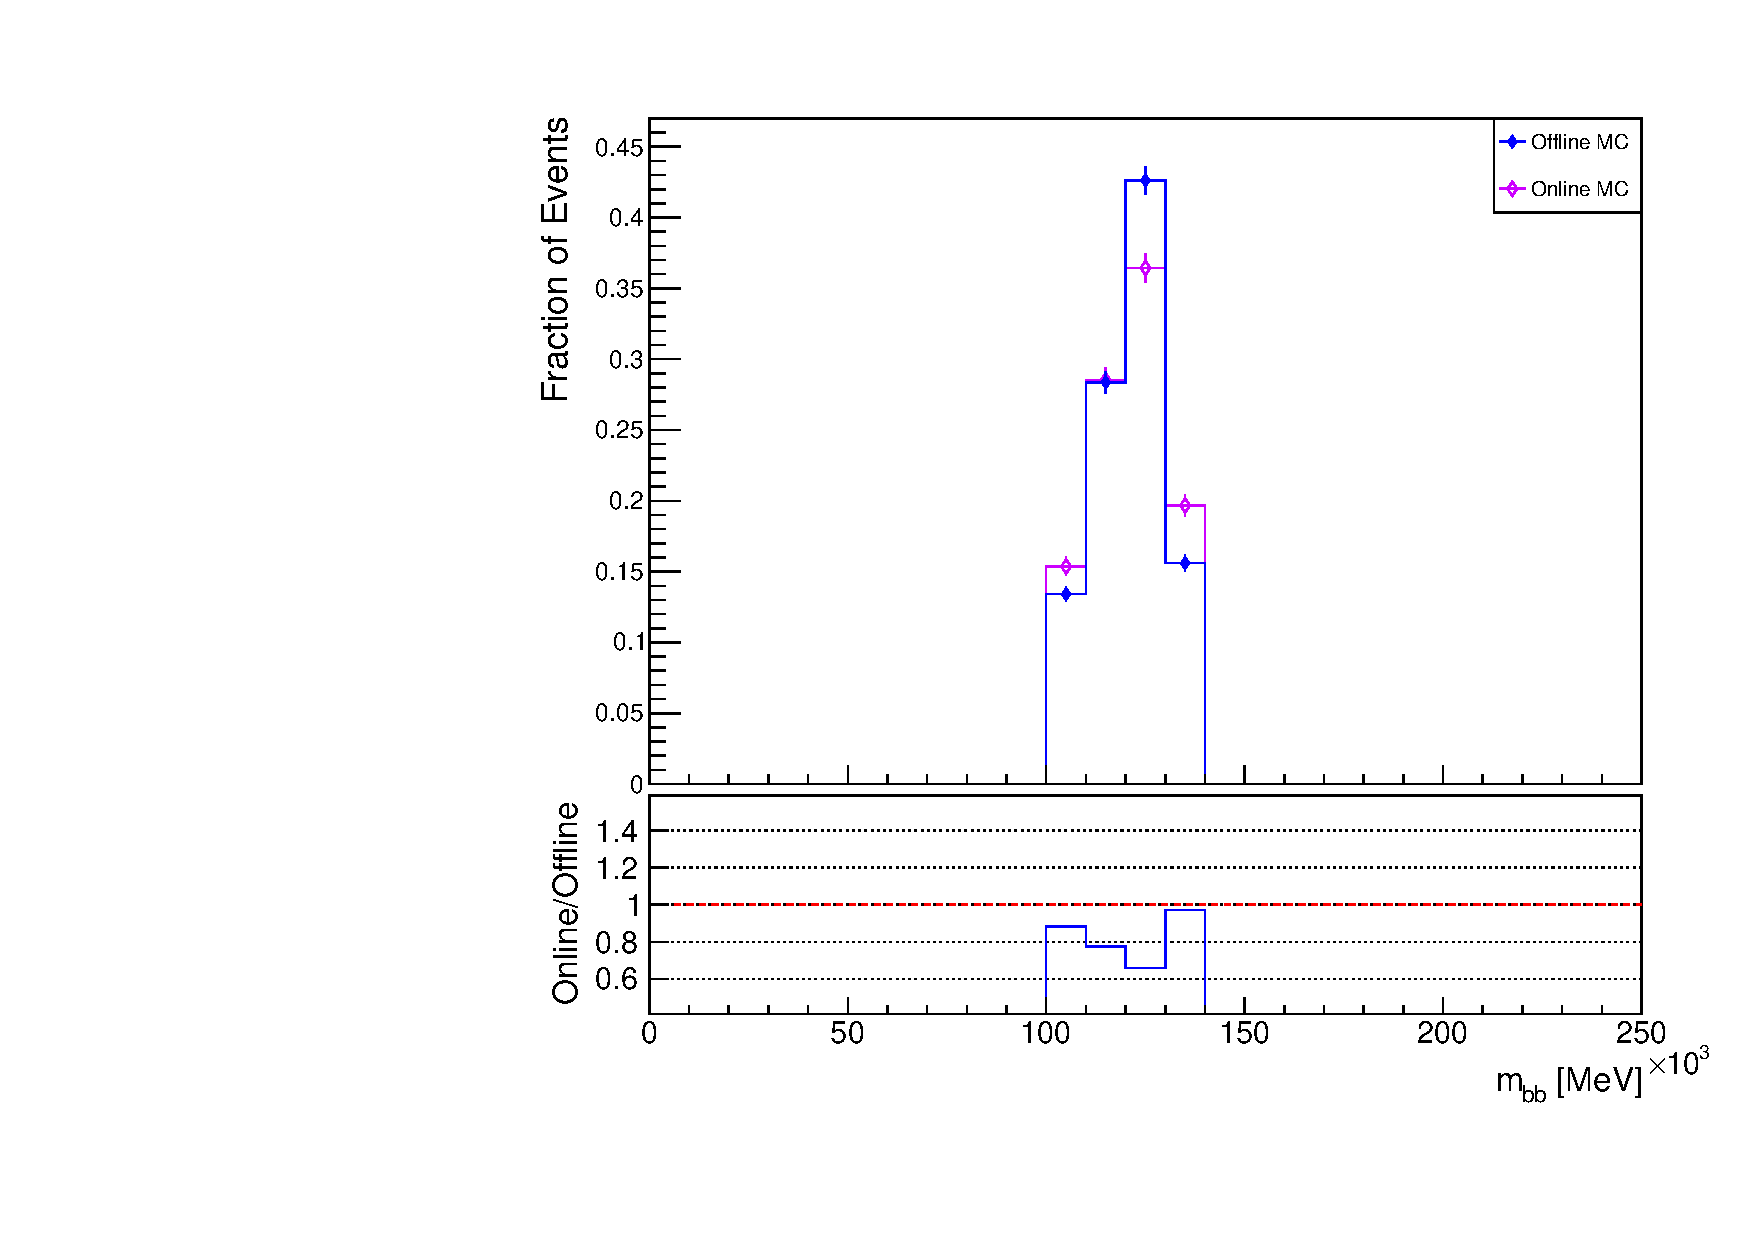
\includegraphics[width=1\linewidth]{mbb_mc_}
			\end{minipage}
			\label{f:mbb}
			\caption[Comparison of the \mbb distribution of the \VBFHBB\ events for HLT and offline objects]{\mbb distribution for the online and offline \VBFHBB\ events, with background events from data shown in the left panel and Monte-Carlo signal events in the right.}
		\end{figure}


\section{BDT Input Variables}

	As discussed in Section \ref{es:as}, the full BDT analysis of the \VBFHBB\ search described in Appendix \ref{a:bdt} was not performed for this dissertation. Given this is a critical component of the full Higgs search \cite{VBFHbb8tev} in \VBFHBB, the performance of select BDT variables is explored for the signal and background regions described in Table \ref{t:signalback}. The variables \mjj and \ptjj covered in the previous section are both BDT training variables.

	This section covers $\eta^*$, given by

	\begin{equation}
	\eta^* = \frac{1}{2}(|\eta_{j1}| + |\eta_{j2}| - |\eta_{b1}| - |\eta_{b2}|)
	\end{equation}

	which is plotted in Figure \ref{f:etastar} for the online and offline events, and the \pt \textit{balance}, given by

	\begin{equation}
		p_{\text{T} balance} = \frac{\vec{p_{\text{T}j1}} + \vec{p_{\text{T}j2}} + \vec{p_{\text{T}b1}} + \vec{p_{\text{T}b2}}}{p_{\text{T}j1} + p_{\text{T}j2} + p_{\text{T}b1} + p_{\text{T}b2}}
	\end{equation}

	which is shown in Figure \ref{f:ptbalance}

	\begin{figure}[h]
		\centering
		\begin{minipage}[h]{0.48\linewidth}
			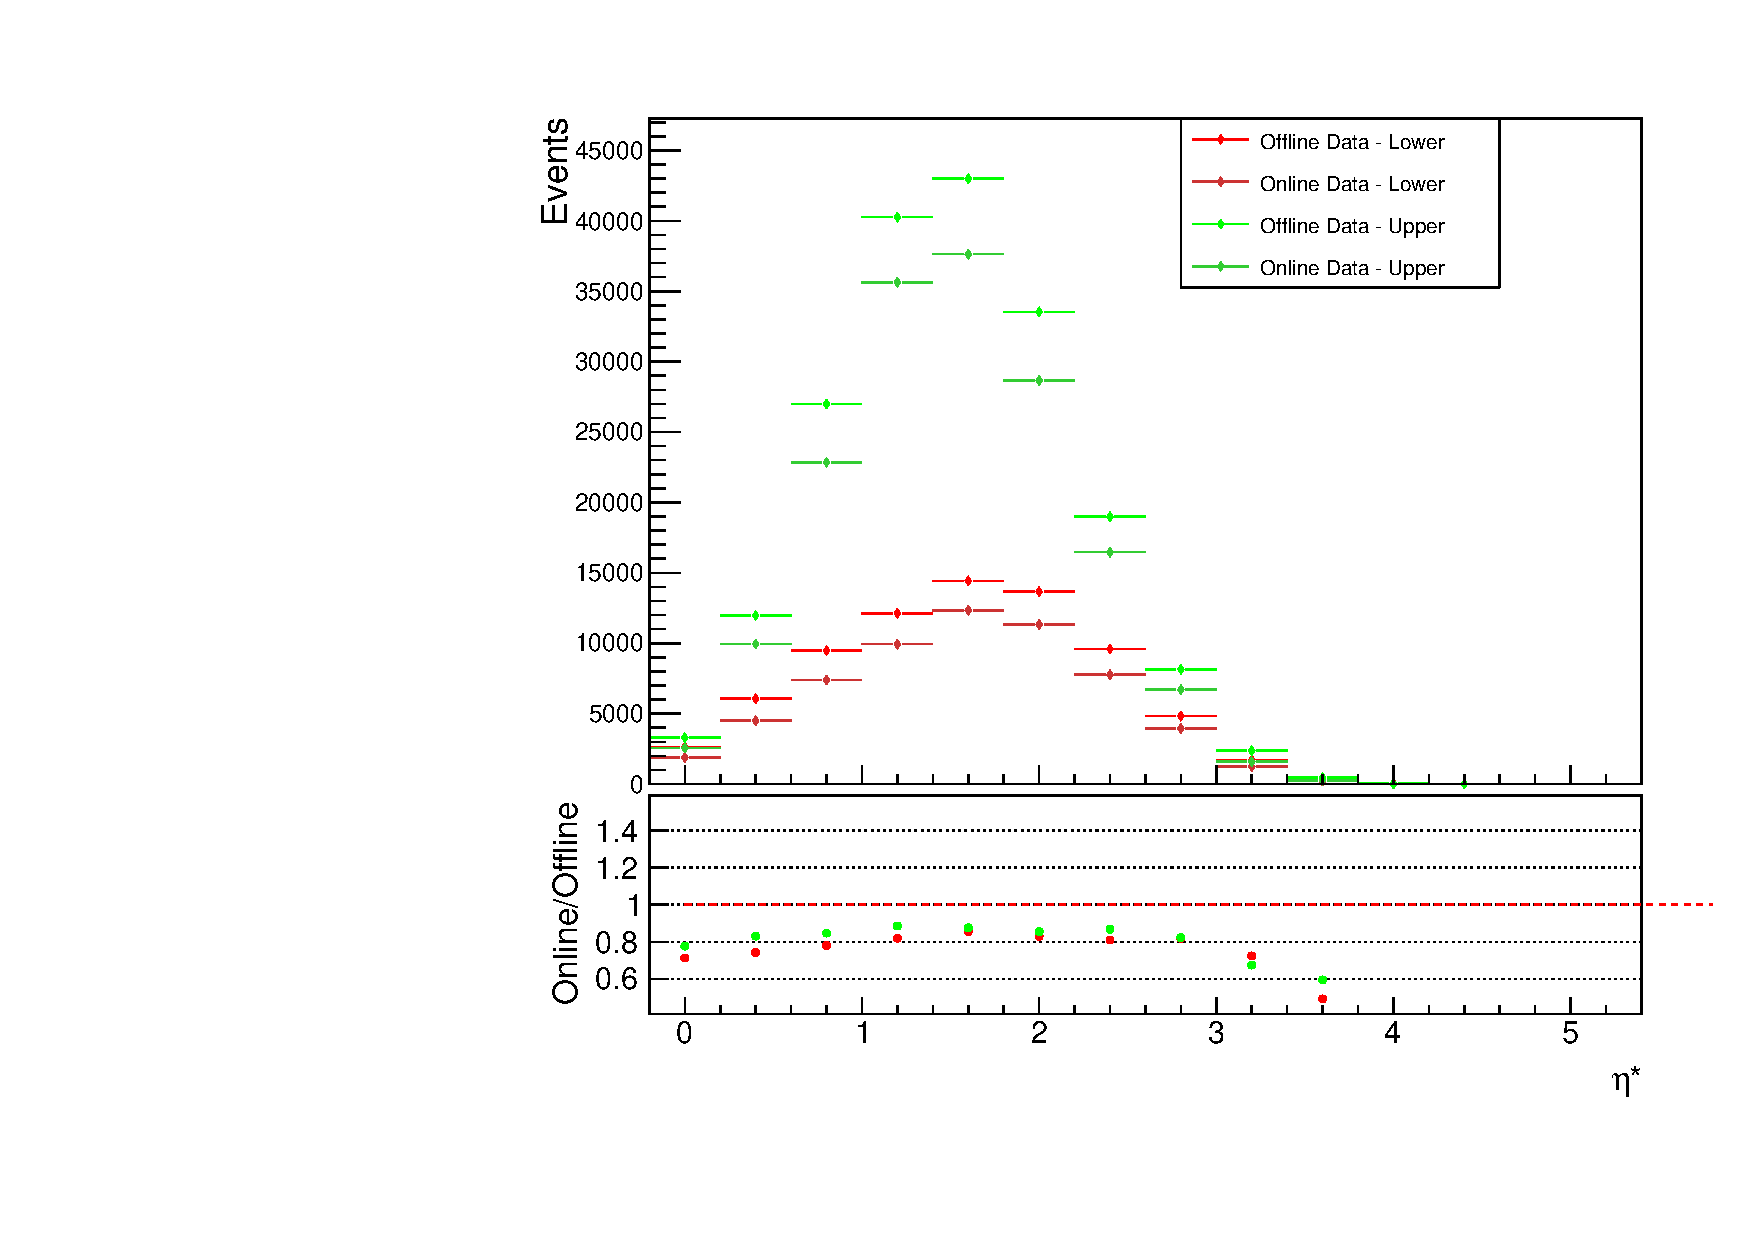
\includegraphics[width=1\linewidth]{etastar_data_}
		\end{minipage}
		\quad
		\begin{minipage}[h]{0.48\linewidth}
			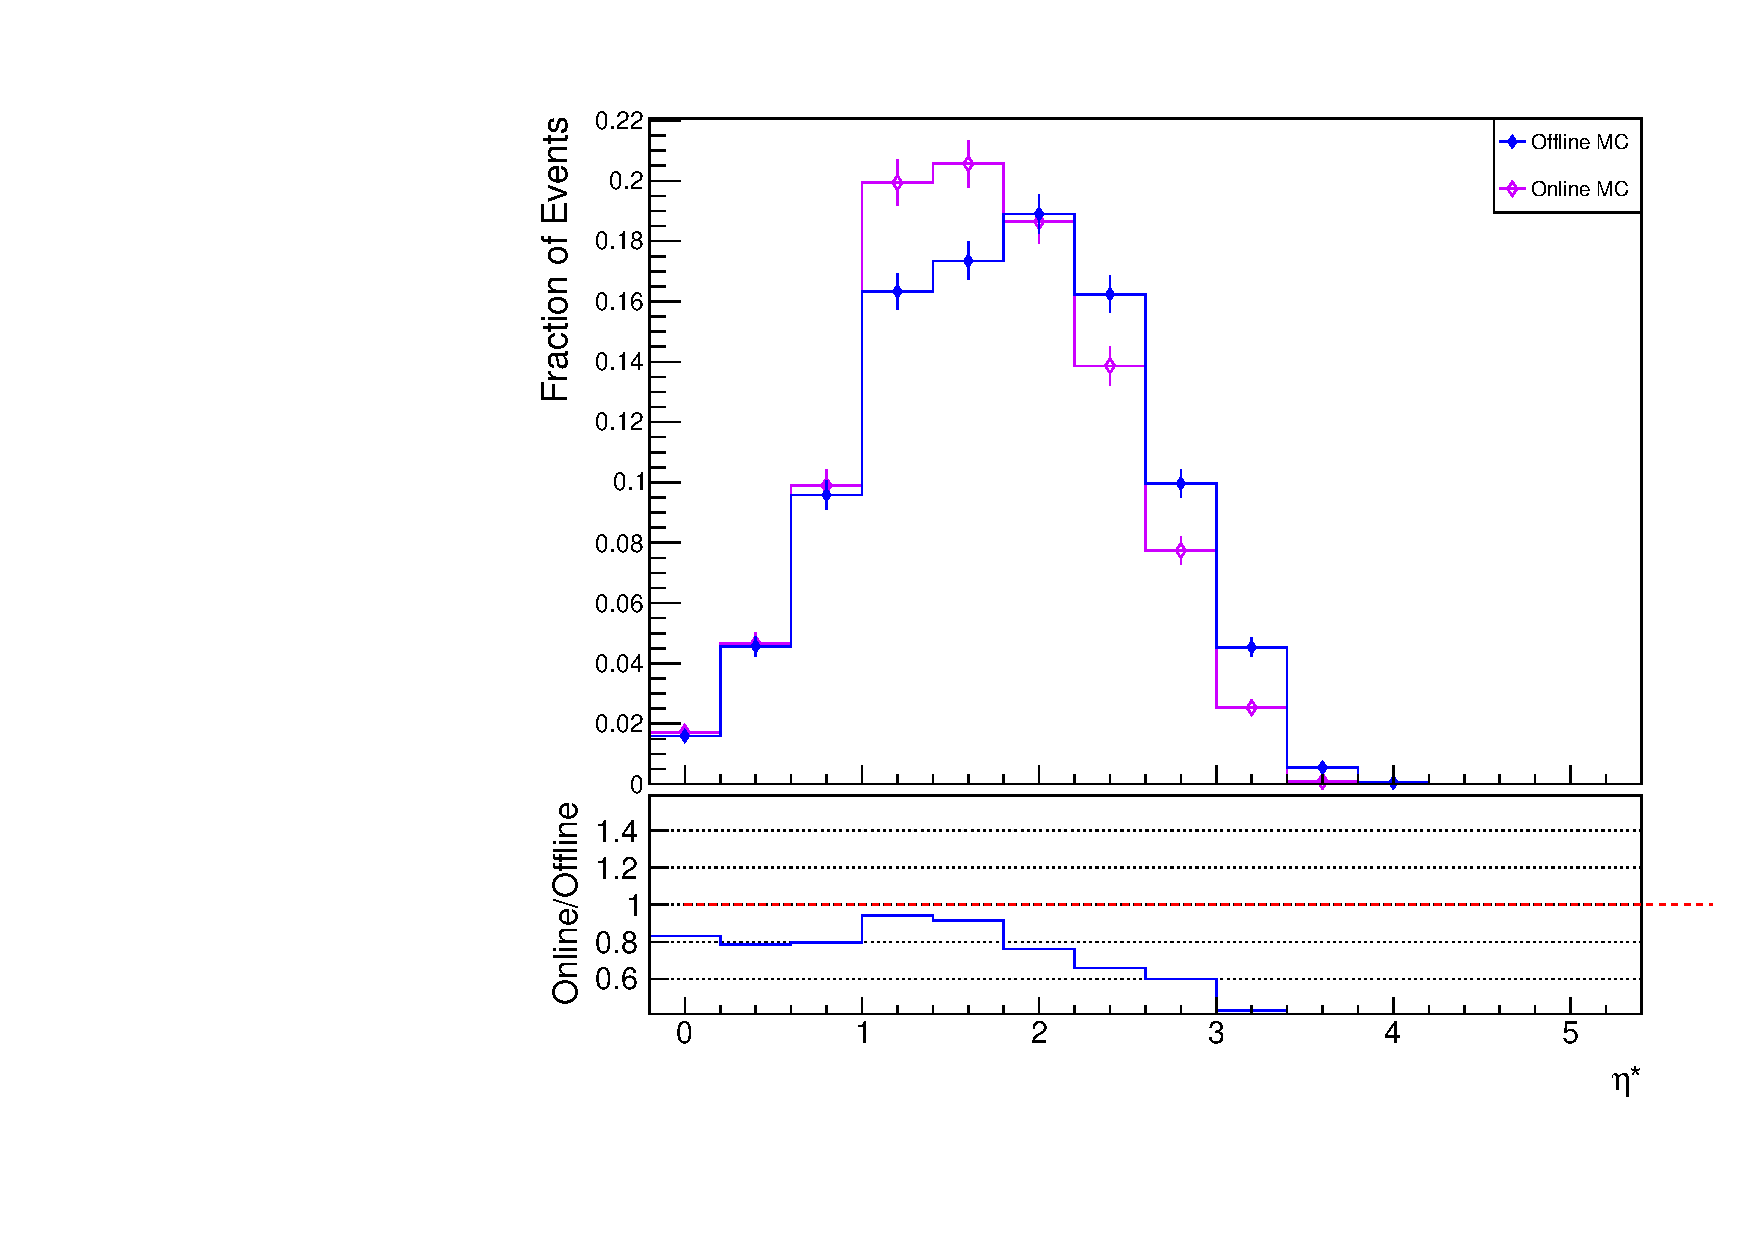
\includegraphics[width=1\linewidth]{etastar_mc_}
		\end{minipage}
		\label{f:etastar}
		\caption[Comparison of the $\eta^*$ distribution of the \VBFHBB\ events for HLT and offline objects]{$\eta^*$ distribution for the online and offline \VBFHBB\ events, with background events from data shown in the left panel and Monte-Carlo signal events in the right.}
	\end{figure}

	\begin{figure}[h]
		\centering
		\begin{minipage}[h]{0.48\linewidth}
			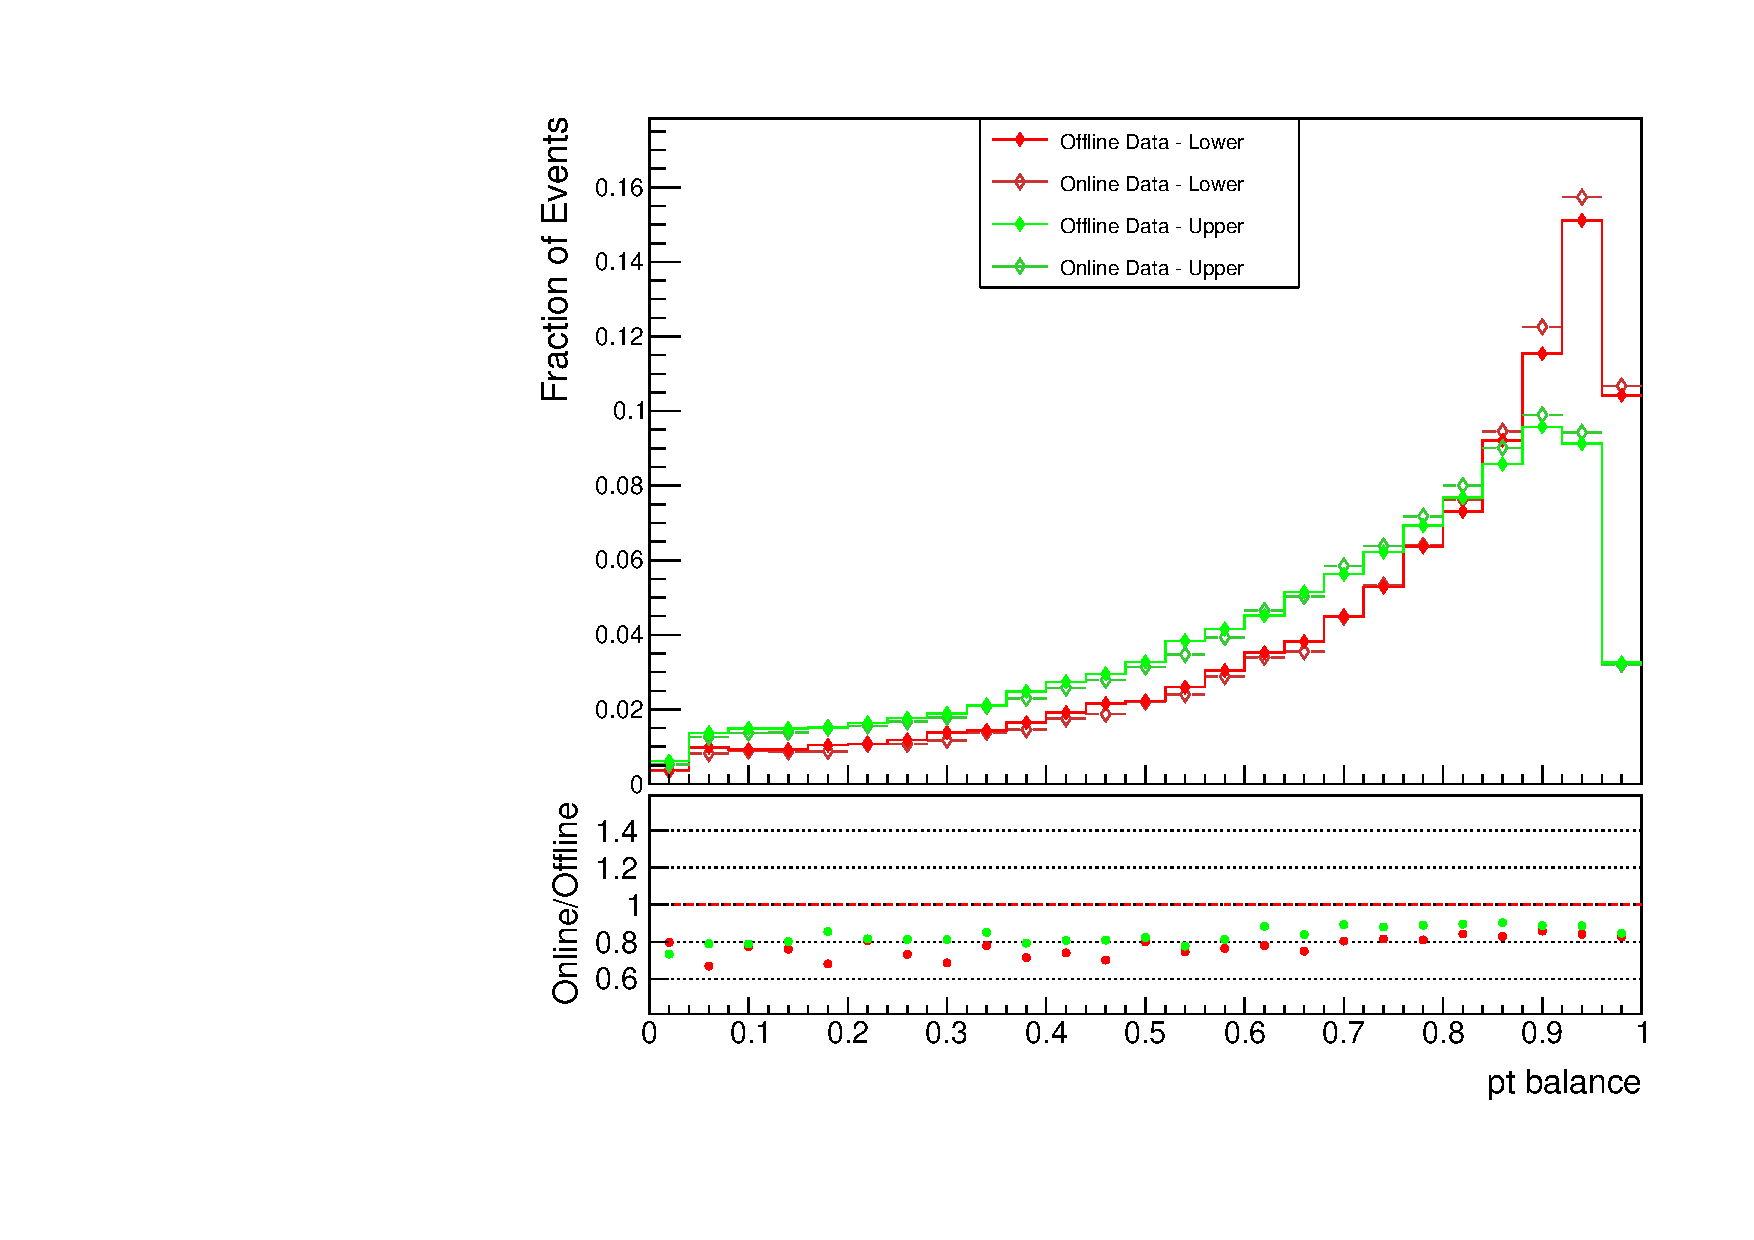
\includegraphics[width=1\linewidth]{ptbalance_data_}
		\end{minipage}
		\quad
		\begin{minipage}[h]{0.48\linewidth}
			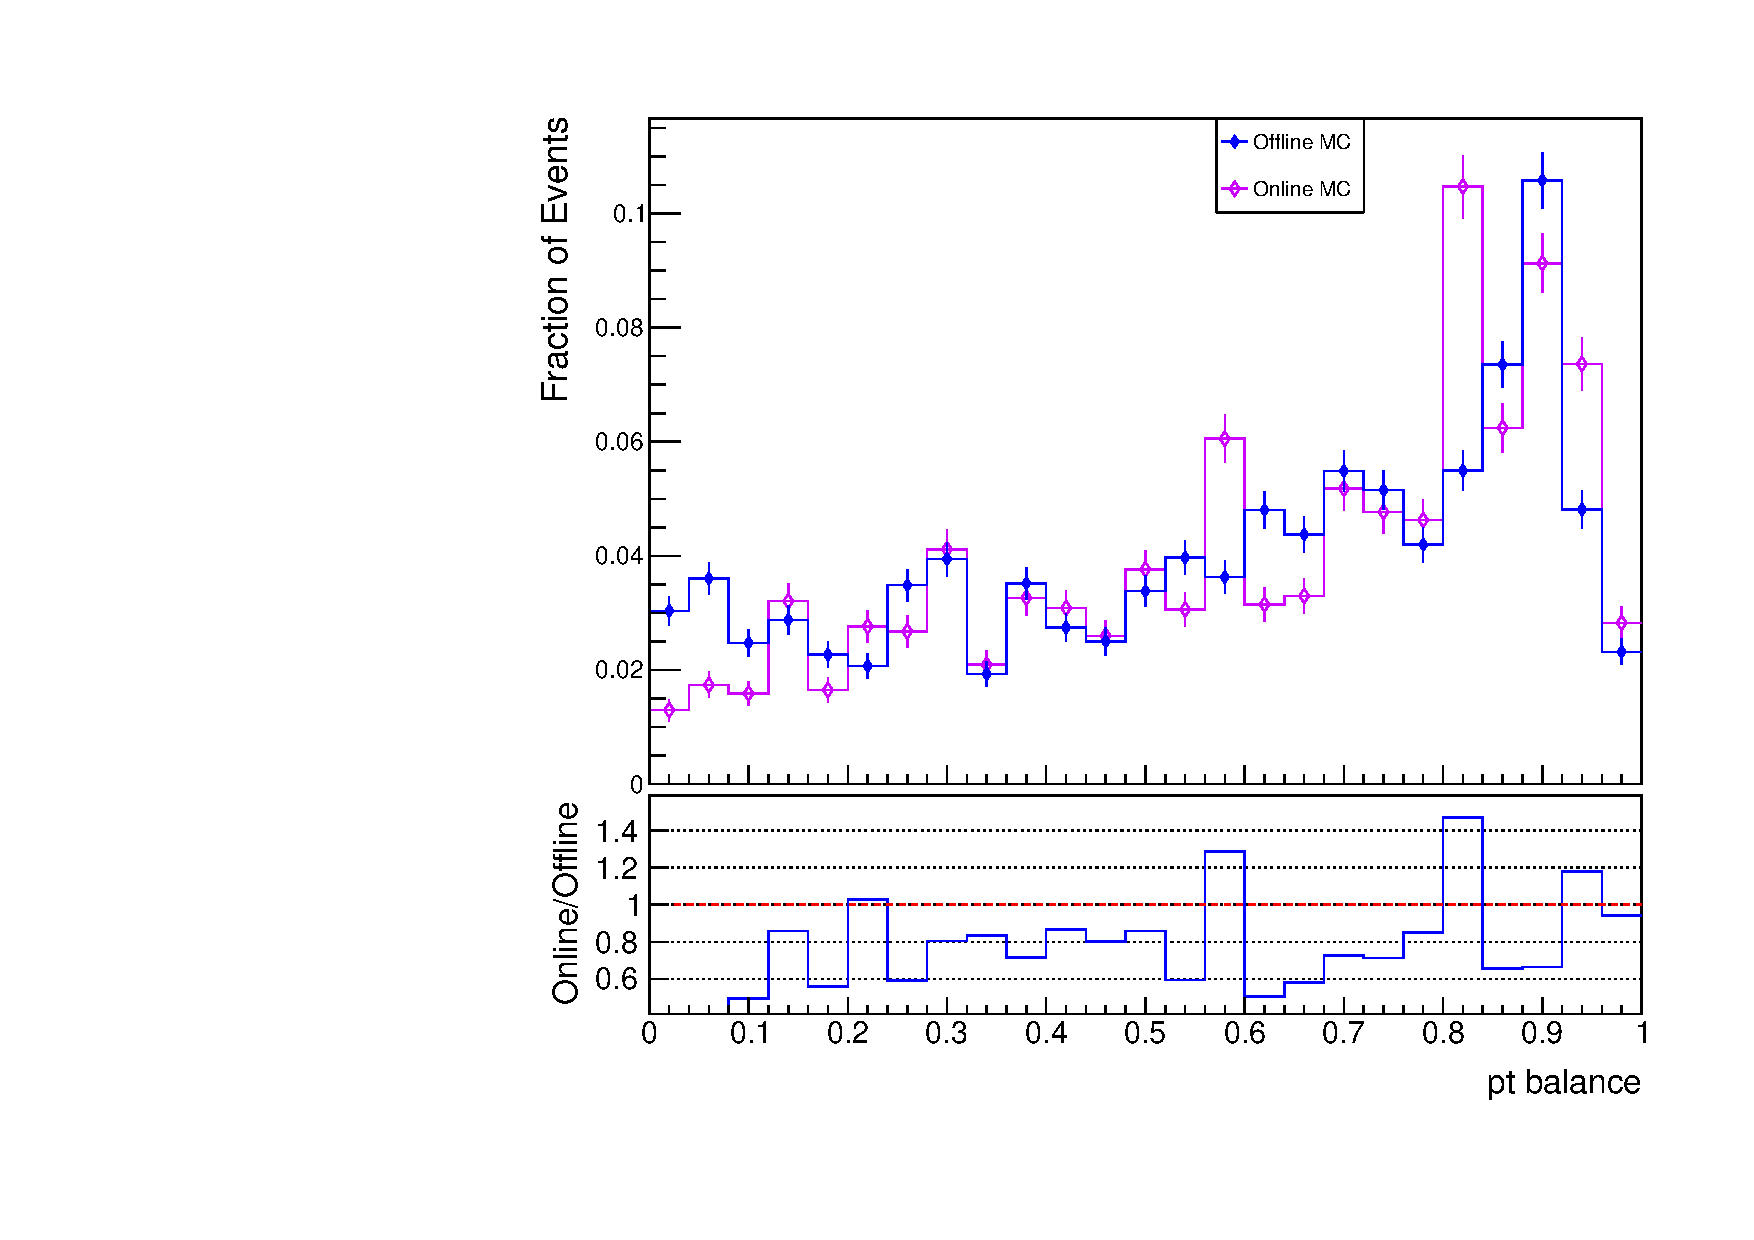
\includegraphics[width=1\linewidth]{ptbalance_mc_}
		\end{minipage}
		\label{f:ptbalance}
		\caption[Comparison of the $p_{\text{T} balance}$ distribution of the \VBFHBB\ events for HLT and offline objects]{$p_{\text{T} balance}$ distribution for the online and offline \VBFHBB\ events, with background events from data shown in the left panel and Monte-Carlo signal events in the right.}
	\end{figure}

	As for the \VBFHBB\ jet kinematic quantities in Section \ref{k:jets}, these variables behave in the same fashion. For the lower background, upper background and signal sectors the shapes of the online and offline curves are comparable. The relative ratio of the online to the offline events is $\0.8$, as covered in Section \ref{k:cutflow} and shown clearly by the ratio plots in the left panels of Figures \ref{f:etastar} and \ref{f:ptbalance}. The plots for the Monte-Carlo signal are noisier, but show a rough $20\%$ decrease in online events compared to offline, and in general the upper background region performs better than the lower region.

	Given this consistent behaviour for the BDT quantities derived from the \VBFHBB\ event, the trigger-level objects should perform comparably to the offline objects, and as such can be used to train a BDT to refine the analysis into a \VBFHBB\ phase space using solely trigger-level objects.

	\section{Summary}

	This chapter presents analysis and comparison of the \VBFHBB\ events attained using trigger-level objects and offline reconstructions in data and Monte-Carlo simulation. The cutflows of the analysis for Monte-Carlo online, Monte-Carlo offline, data online and data offline were studied, and found to show online analysis produced $\sim82\%$ of the results of offline analysis for Monte-Carlo simulations, and $\sim84\%$ for data.

	While this is a reduction of event yield for a given analysis sample, the increased trigger rates permitted when applying TLA will result in an increased final event count even given the decrease in efficiency. For current rate increases in TLA analyses \cite{tla}, this would amount to an increase of $\sim66\%$ in the final number of events. This estimate of the possible increase does not take into account any limitations on the rate that may result from increased computational demands on either processing or TLA object byte size.

	To confirm that the TLA analysis would be possible with the trigger-level objects, the component jets, kinematic properties of the \VBFHBB\ event and select BDT training variables were investigated. These cases showed consistent behaviour between the online and offline objects in both background data and signal Monte-Carlo simulation, while showing the online rate decrease calculated from the cutflows.

	These suggests a full study of \VBFHBB\ analysis is a feasable proposal. Use of TLA could increase the output rate of the tirggers to statistically significant levels and the objects produced will behave during analysis in a consistent fashion to the offline objects.
\endinput
